%*****************************************
\chapter{\textbf{Model and Samples}} \label{ch: Model}
%*****************************************
\vspace{0.5cm} 

%============================================================================================================================================================
\section{Introduction}

In this chapter, we present an analysis of the occurrence of exoplanetary ringed systems. The first step consists in proposing a probability for the transits based on five different probabilities: the probability of a star harboring a planet in orbit, the probability of this planet having material around which could coalesce and form rings, the probability of observing the transit giving general geometric constraints, the probability of observing at least one transit during the nominal five-year \textit{Gaia} mission, and the probability of rings around a planet to be present at the moment of the observations. In order to solve this, we proposed a Monte-Carlo approach in which the most important parameters involved in this probability are simulated as could be the stellar mass and the planetary mass-period distributions. These distributions follow regular power laws making the Monte-Carlo suitable for our purpose. On the other hand, as we also count with an analytic function the same process was addressed and compared to the Monte-Carlo results.\\

The section is organized as follows: in \autoref{sec:PowerLawSec} the basis of the power law and Monte-Carlo approach is presented. The application of this method to planetary mass-period distribution and stellar IMF is addressed in \autoref{ref:PM_ExoPlanet} and \autoref{sec:StellarMAS_IMF} . Finally, in \autoref{sec:DetectionProbability} the proposed solution and comparison between the Monte-Carlo and the analytic approaches is presented. 

%============================================================================================================================================================

%============================================================================================================================================================
\section{Power Law Distributions} \label{sec:PowerLawSec}

It is well-known that the stellar mass, and exoplanetary mass and orbital period distributions can be described by power laws. As those parameters are essential in our formulation for the probability of exoplanetary rings transits, and the subsequent analysis, we must pay attention to how model samples which can reproduce faithfully the observation.\\

%A power law distribution can be defined as the relative change of two quantities, which are related through a common exponent. In other words, we can predict the change in one of the variables once the exponent and an initial set of values for the second variable are known. 
A power law distribution is defined as a functional relationship of a variable $N$ as a function of a variable $X$. The relative change in one of the variables induces a change in the other, modulated by one of the variables to a given power.   
Mathematically speaking, we define a power law distribution as \autoref{eq:PowerLaw}, where $N$ and $X$ are the variables, and $\alpha$ is the exponent relating the relative change between them and it is assumed $\alpha \neq 1$. Generally, the variable $N$ refers to the number of objects one would expect to find in a given interval $x_1 \leq X \leq x_2$, where the variable $X$ in our particular case may refer to the planetary period, planetary mass, stellar mass or any other parameter which we want to study.\\ 

\begingroup
\Large
\begin{equation}
 \frac{\textnormal{dN}}{\textnormal{dX}}~~\propto~~\textnormal{X}^{-\alpha}
 \label{eq:PowerLaw}
\end{equation}
\endgroup\\

%Power-laws can consist of a single or multiple exponents relating two or more variables. 
Power-laws can have single or multiple components described by different exponents. The easiest case is the single power law which has the mathematical form shown in \autoref{eq:PowerLaw}. However, the equation lacks a proportionality constant or normalization constant which must be found with boundary conditions. Therefore, \autoref{eq:PowerLaw} can be rewritten in a more general fashion as \autoref{eq:PowerLaw_1}, where $A$ corresponds to the normalization constant and can be found using \autoref{eq:NormConst} with $\gamma = 1 - \alpha$.\\

\begingroup
\Large
\begin{equation}
 \frac{\textnormal{dN}}{\textnormal{dX}}~~=~~\frac{\textnormal{X}^{-\alpha}}{A}~~~~~~~;~~~~~~~x_1 ~~\leq ~~\textnormal{X}~~ \leq ~~\textnormal{x}_2
 \label{eq:PowerLaw_1}
\end{equation}
\endgroup\\

\begingroup
\Large
\begin{equation}
 \textnormal{A}~~=~~\int_{\textnormal{x}_1}^{\textnormal{x}_2} X^{-\alpha} \textnormal{dX}~~=~~\frac{\textnormal{x}_2^{1 - \alpha} - \textnormal{x}_1^{1 - \alpha}}{1 - \alpha}~~=~~\frac{\textnormal{x}_2^{\gamma} - \textnormal{x}_1^{\gamma}}{\gamma} 
 \label{eq:NormConst}
\end{equation}
\endgroup\\

Furthermore, we can define the cumulative distribution function (CDF) $F(X)$, which will give us all the accumulated probability less than or equal to $X$. It is widely used to determine the probability of an observation being greater than a certain value, or between two values. The CDF will be of great importance in \autoref{sec:MCSec} where the randomly distributed variable is obtained by making use of it to generate the real variable. The mathematical form of the CDF is given in \autoref{eq:CDF} where the upper limit in the integral $x$ here refers to a value between the upper limit ($x_1$) and lower limit ($x_2$) over which one wants to generate the distribution.\\ 

\begingroup
\Large
\begin{equation}
 \textnormal{F}(\textnormal{x})~~=~~\textnormal{A}^{-1} \int_{\textnormal{x}_1}^{\textnormal{x}} \textnormal{t}^{-\alpha} \textnormal{dt}~~=~~\frac{\textnormal{x}^{\gamma} - \textnormal{x}_1^{\gamma}}{\textnormal{x}_2^{\gamma} - \textnormal{x}_1^{\gamma}}
 \label{eq:CDF}
\end{equation}
\endgroup\\

Subsequently, if the random variable is distributed uniformly between $0$ and $1$, one can generate the real variable by inverting the CDF shown in \autoref{eq:CDF} which leads to \autoref{eq:RandomVar}. As expected, if one evaluates the last equation in $y = 0$ and $y = 1$ which are the extreme values of the random variable, the result is $x = x_1$ and $x = x_2$ respectively in the real variable.\\

\begingroup
\Large
\begin{equation}
  \begin{align*}
    \textnormal{y} & ~~=~~  \textnormal{F}(\textnormal{x}) ~~=~~ \frac{\textnormal{x}^{\gamma} - \textnormal{x}_1^{\gamma}}{\textnormal{x}_2^{\gamma} - \textnormal{x}_1^{\gamma}} \\[10pt]
    \textnormal{x} & ~~=~~  (y~ (~\textnormal{x}_2^{\gamma} - \textnormal{x}_1^{\gamma}~) + \textnormal{x}_1^{\gamma})^{1/\gamma}
    \label{eq:RandomVar}
  \end{align*}
\end{equation}
\endgroup\\

The planetary mass-period distribution, and the stellar mass distribution will be generated following the simple power law explained above with a Monte-Carlo process in \autoref{sec:MCSec}. Although a different method was also explored for the planetary mass-period distribution due to a possible weakly dependence in both parameters (\cauthor{1538-3881-134-5-2061} \citeyear{1538-3881-134-5-2061}; \cauthor{2002ApJ...568L.113Z} \citeyear{2002ApJ...568L.113Z}), we decided to keep the power law method to model them as it is also widely used and studied in literature (\cauthor{2010EAS....41..107N} \citeyear{2010EAS....41..107N}; \cauthor{2008PASP..120..531C} \citeyear{2008PASP..120..531C}; \cauthor{2006ApJ...646..505B} \citeyear{2006ApJ...646..505B}).  

\section{Exoplanets: Period-Mass Distributions} \label{ref:PM_ExoPlanet}

In order to draw a reliable distribution sample of period and mass for exoplanets, we used two different approaches. The first approach uses the $\beta$-distribution because there exists a correlation between the period and mass of an exoplanet as shown by \cauthor{2002ApJ...568L.113Z} (\citeyear{2002ApJ...568L.113Z}). This makes the distribution analysis not suitable to be addressed by two independent power laws in order to describe the joint period-mass distribution. Alternatively, one can assume that as the correlation is weak, then each variable can be treated as independent and the distributions may be generated using single power laws as it is also widely explored by other authors \cauthor{2010EAS....41..107N} (\citeyear{2010EAS....41..107N}). Therefore, as there exist two different forms to address the generation of these distributions, both ways were explored and implemented in this work.\\

In \autoref{subsec:BetaDist} and \autoref{subsec:SPLDist}, the method is widely explained taking into account the different observations and arguments as shown in \cauthor{2002ApJ...568L.113Z} (\citeyear{2002ApJ...568L.113Z}) and \cauthor{2010EAS....41..107N} (\citeyear{2010EAS....41..107N}). 

\subsection{\texorpdfstring{$\beta$-}Distribution} \label{subsec:BetaDist}

Using a dataset of 66 exoplanets \cauthor{2002ApJ...568L.113Z} (\citeyear{2002ApJ...568L.113Z}) explored a possible correlation between the mass and period. Subsequently \cauthor{1538-3881-134-5-2061} (\citeyear{1538-3881-134-5-2061}) using a data set of 233 exoplanets supported this idea measuring a positive correlation coefficient of $0.1762$. As a result of the positive correlation, describing the distribution as two independent power laws it is not correct, and a new coupled positively correlated function is needed to describe the problem. However, generating this type of distributions needs $\beta$-distributed random variables which was not provided until \cauthor{2004CMS...46.397M} (\citeyear{2004CMS...46.397M}) work.\\

The probability distribution function (pdf) on a finite interval (c,d), $-\infty < \textnormal{c} < \textnormal{d} < \infty $, indexed by two positive parameters $\alpha$ and $\beta$ is given by \autoref{eq:BetaPDF}, where $\textnormal{B}(\alpha, \beta)$ denotes the beta function and can be computed using \autoref{eq:BetaExplicit}.\\

\begingroup
\Large
\begin{equation}
 \textnormal{f}_\beta(\textnormal{x} | \alpha, \beta)~~=~~\frac{1}{\textnormal{B}(\alpha, \beta)} \frac{(\textnormal{x}-\textnormal{c})^{\alpha -1} (\textnormal{d}-\textnormal{x})^{\beta -1}}{(\textnormal{d}-\textnormal{c})^{\alpha + \beta - 1}}~~~~~~~;~~~~~~~\textnormal{c}~~ \leq ~~\textnormal{x} ~~\leq ~~\textnormal{d},~~~\alpha>0,~~~\beta>0
 \label{eq:BetaPDF}
\end{equation}
\endgroup

\begingroup
\Large
\begin{equation}
 \textnormal{B}(\alpha, \beta)~~=~~\int_0^1 \textnormal{t}^{\alpha -1}(1-\textnormal{t})^{\beta -1} \textnormal{dt}~~=~~\frac{\Gamma(\alpha)\Gamma(\beta)}{\Gamma(\alpha + \beta)}
 \label{eq:BetaExplicit}
\end{equation}
\endgroup\\

Using the correct transformation, the pdf can be written in terms of a normally distributed random variable `$\textnormal{y}$' to obtain the standard $\beta$-distribution as shown in \autoref{eq:BetaStandard} which is a useful form to implement the algorithm provided in \cauthor{2004CMS...46.397M} (\citeyear{2004CMS...46.397M}).\\    

\begingroup
\Large
\begin{equation}
  \textnormal{f}(\textnormal{y} \mid \alpha, \beta)~~=~~\frac{1}{\textnormal{B}(\alpha, \beta)} \textnormal{y}^{\alpha -1}(1-\textnormal{y})^{\beta-1}~~~~~~~;~~~~~~~\textnormal{0} ~~\leq ~~\textnormal{y} ~~\leq ~~\textnormal{1},
 \label{eq:BetaStandard}
\end{equation}
\endgroup\\

The final distribution for mass and period can be obtained making use of \autoref{eq:FinalDist}, where the marginal distributions of M and P follow the $\beta$-distribution as in \autoref{eq:BetaExplicit}. One can re-write the marginal distributions of the random variables as in \autoref{eq:CorrelatedPairs} and define two new variables $\delta_1$ and $\delta_2$ following the standard $\beta$-distribution and relate them through the correlation coefficient $\rho(\textnormal{M}_1), \rho(\textnormal{P}_1)$. Thus, if one wants to reproduce the probability distribution of two variables correlated in this fashion, first a marginal distribution must be assumed for $\textnormal{M}_1$ and $\textnormal{P}_1$ and using the maximum likelihood method, the best estimation $(\hat{\alpha_m},\hat{\beta_m})$ of $(\alpha_m,\beta_m)$, and $(\hat{\alpha_p},\hat{\beta_p})$ of $(\alpha_p,\beta_p)$ can be obtained. The correlation coefficient can be computed $\hat{\rho}(\textnormal{M}_1), \rho(\textnormal{P}_1)$ to be used as the value for $\rho(\textnormal{M}_1), \rho(\textnormal{P}_1)$ which allows to generate pairs of $\textnormal{M}_1$ and $\textnormal{P}_1$ using \autoref{eq:CorrelatedPairs}, where $\textnormal{G}(\alpha)$ is a random variable distributed as a $\Gamma$-distribution.\\   

\begingroup
\Large
\begin{equation}
    \textnormal{f}(M, P | \alpha_m, \beta_m,\alpha_p, \beta_p )
    \label{eq:FinalDist}
\end{equation}
\endgroup

\begingroup
\Large
\begin{equation}
  \begin{align*}
    \textnormal{M}_1~~ &=~~  \frac{\textnormal{M} - \textnormal{m}_1}{\textnormal{m}_2 - \textnormal{m}_1} ~~&= ~~\frac{\textnormal{G}(\alpha^*_m)+\textnormal{G}(\delta_1)}{\textnormal{G}(\alpha^*_m)+\textnormal{G}(\delta_1)+\textnormal{G}(\beta^*_m)+\textnormal{G}(\delta_2)}\\[10pt]
    \textnormal{P}_1 ~~&= ~~\frac{\textnormal{P} - \textnormal{p}_1}{\textnormal{p}_2 - \textnormal{p}_1} ~~&=~~ \frac{\textnormal{G}(\alpha^*_p)+\textnormal{G}(\delta_1)}{\textnormal{G}(\alpha^*_m)+\textnormal{G}(\delta_1)+\textnormal{G}(\beta^*_p)+\textnormal{G}(\delta_2)}
    \label{eq:CorrelatedPairs}
  \end{align*}
\end{equation}
\endgroup\\

Applying this algorithm and using the observed data the parameters can be set to $(\hat{\alpha}_m, \hat{\beta}_m) = (0.6524, 5.9070)$ and $(\hat{\alpha}_p, \hat{\beta}_p) = (0.3697, 3.8445)$ as a result of applying a Maximum-Likelihood Method. Thus, one can rewrite the distributions as shown in \autoref{eq:FinalDist_2} where the normalization constants in both cases are given by $A_1 = 115.5$ and $A_2 = 11650$, corresponding to the area below the observed histogram distribution for each one of the parameters.

\begingroup
\Large
\begin{equation}
  \begin{align*}
    \textnormal{f}_\beta^{\textnormal{M}}~~ & = ~~\textnormal{A}_1\textnormal{f}_\beta(\textnormal{m}|\hat{\alpha}_m, \hat{\beta}_m) \\[10pt]
    \textnormal{f}_\beta^{\textnormal{P}}~~ & = ~~\textnormal{A}_2\textnormal{f}_\beta(\textnormal{p}|\hat{\alpha}_p, \hat{\beta}_p)
    \label{eq:FinalDist_2}
  \end{align*}
\end{equation}
\endgroup\\

In short, the mass and period distributions can be then generated using \autoref{eq:BetaStandard} and \autoref{eq:FinalDist} through a Monte-Carlo process. These equations can be read as the probability of a planet to be in a mass range $[M, M + dM]$ and a period range $[P, P + dP]$. The actual upper and lower limits in mass, and period are given by the data set used to derive the normalization constant and the index of the $\beta$-distribution. Thus, we can generate samples in mass-period ranges of $0.008 < M(M_j) < 26.7$ and $0.8079 < P(days) < 6776.1$. The application of this model to our current problem is shown and discussed in \autoref{sec:MCSec}.

\subsection{Single Power-Law} \label{subsec:SPLDist}

As discussed in \autoref{sec:PowerLawSec} and \autoref{subsec:BetaDist}, the planetary mass and period are weakly correlated, so one can ignore that fact and address the problem as independent single power laws. In the past, this has been studied by (\cauthor{2008PASP..120..531C} \citeyear{2008PASP..120..531C}; \cauthor{2006ApJ...646..505B} \citeyear{2006ApJ...646..505B}) considering the distributions of semi-major axis and planet mass of known exoplanets. However, in recent studies, \cauthor{2010EAS....41..107N} (\citeyear{2010EAS....41..107N}) noted that due to a decrease in sensitivity of the radial velocity method with the orbital distance the exponent of the distribution must be modified. The single power law distributions in mass, semi-major axis and period proposed are shown in \autoref{eq:MassPeriodDist}.\\

\begingroup
\Large
\begin{equation}
  \begin{align*}
    \frac{\textnormal{dN}}{\textnormal{dm}}~~&\propto~~\textnormal{m}^{-1.16} \\[10pt]
    \frac{\textnormal{dN}}{\textnormal{da}}~~&\propto~~\textnormal{a}^{-0.61} \\[10pt]
    \frac{\textnormal{dN}}{\textnormal{dP}}~~&\propto~~\textnormal{P}^{-0.74}
    \label{eq:MassPeriodDist}    
 \end{align*}
\end{equation}
\endgroup\\

In the same way as stated before, we can interpret the former equations as the number of planets expected to be contained in a mass range $m_1 < m < m_2$, a semi-major axis range $a_1 < a < a_2$, and orbital period $p_1 < p < p_2$. Whereas in the case of $\beta$-distributions, the mass covers a wide range of $\sim0.008-26.7~M(M_j)$, the period's range is valid only in $\sim0.8079-6776.1~\textnormal{days}$, which leads to a semi-major axis limit of $\sim0.0169-7~\textnormal{AU}$. However, using the power law distributions allows us to use a reduced mass range of $0.5 < M(M_j) < 13$, still suitable for our purpose, but with an upper cut-off at $75 AU$ which leads to an upper limit of $\sim 650$yr in the period including wider planetary orbits.    

\section{Stellar Mass Distribution}\label{sec:StellarMAS_IMF}

Apart from modeling the planetary mass and period, we aimed to obtain in the same fashion the stellar mass distribution. This is known as the initial mass function (IMF) and it is still a wide-open question in current Astrophysics. There exist different power laws which try to describe the number of stars expected to lie in a given mass range. In this work, we decided to test two different forms of the IMF namely the Salpeter power law proposed by Edwin Salpeter in $1955$ \cauthor{1955ApJ...121..161S} (\citeyear{1955ApJ...121..161S}) and the Kroupa power law proposed by Pavel Kroupa in $2001$ \cauthor{2001MNRAS.322..231K} (\citeyear{2001MNRAS.322..231K}). The main difference between these two formulations resides on the value that each exponent can take according to each mass range in which one could be interested in. The main goal in using these power laws is to faithfully reproduce the actual observed IMF distribution of stars in a given mass range using the Monte-Carlo process technique. In \autoref{subsec:Salpeter} and \autoref{subsec:Kroupa} a brief introduction of the main features for both power laws is given.    

\subsection{Salpeter Power-Law} \label{subsec:Salpeter}

In 1955, Edwin Salpeter used the observed luminosity function for main-sequence stars in the solar neighborhood assuming that stars off the main-sequence have already burnt up $~10\%$ of their hydrogen mass, and also that stars in the solar neighborhood have been created at a uniform rate for the last five billion years to compute the rate of star creation as a function of stellar mass, and the number of stars in each mass range \cauthor{1955ApJ...121..161S} (\citeyear{1955ApJ...121..161S}). Having said that, he found the power law describing the IMF follows \autoref{eq:Salpeter_1}, in which $\xi_0$ is a constant related to the local stellar density and $\alpha = 2.35$. The former equation gives us the number of stars expected to be in a mass range $[M$, $M + dM]$.\\ 

\begingroup
\Large
\begin{equation}
  \xi(\textnormal{m})\Delta \textnormal{m} = \xi_0 \left(\frac{\textnormal{m}}{\textnormal{M}_\odot} \right)^{-2.35} \left(\frac{\Delta \textnormal{m}}{\textnormal{M}_\odot} \right)
 \label{eq:Salpeter_1}
\end{equation}
\endgroup\\

As we are interested in using our own mass range, and just make use of the exponent to draw a mass distribution we can rewrite \autoref{eq:Salpeter_1} into \autoref{eq:Salpeter_2}, and later apply all the steps listed in \autoref{sec:PowerLawSec} to later make use of the Monte-Carlo process and obtain our sample of modeled stars. The proportionality constant can be found once the total number of stars in a mass range $m_1 < m < m_2$ is known, through \autoref{eq:NormConst}.

\begingroup
\Large
\begin{equation}
  \frac{\textnormal{dN}}{\textnormal{dm}} \propto m^{-2.35}
 \label{eq:Salpeter_2}
\end{equation}
\endgroup\\

\subsection{Kroupa Power-Law} \label{subsec:Kroupa}

On the other hand, in $2001$, a different formulation was proposed by Pavel Kroupa in which the main feature is a change in the slope (power-law index) near to $0.08M_\odot$ and $0.5M_\odot$ \cauthor{2001MNRAS.322..231K} (\citeyear{2001MNRAS.322..231K}). In other words, the number of stars expected in a given mass range has different values for the power-law exponent in contrast to Salpeter's law which has only one index. The general form is given by \autoref{eq:Kroupa_1}. One interesting feature of this power law is that $50\%$ of the data generated falls into the mass range $0.01 \leq \frac{m}{M_\odot} \leq 1.0$, and $50\%$ falls into $1.0 \leq \frac{m}{M_\odot} \leq 50.0$. 

\begingroup
\Large
\begin{equation}
    \xi(\textnormal{m}) \propto m^{-\alpha_0} = 
    \begin{cases}
     \alpha_0 = +0.3 \pm 0.7,& \text{if } ~~ 0.01 \leq \frac{m}{M_\odot} \leq 0.08\\
     \alpha_0 = +1.3 \pm 0.5,& \text{if } ~~ 0.08 \leq \frac{m}{M_\odot} \leq 0.50\\
     \alpha_0 = +2.3 \pm 0.3,& \text{if } ~~ 0.50 \leq \frac{m}{M_\odot} \leq 1.00\\
     \alpha_0 = +3.3 \pm 0.7,& \text{if } ~~ 1.00 \leq \frac{m}{M_\odot}
    \end{cases}
\label{eq:Kroupa_1}
\end{equation}
\endgroup\\

The IMF generation will be addressed in the same fashion as explained above for the Salpeter's power law, where a Monte-Carlo process will be used and the normalization constant will be set to the total number of stars in a mass range $m_1 < m < m_2$. 

%============================================================================================================================================================
\section{Probability of Transit Detection} \label{sec:DetectionProbability}

%Star with a planet, Gaia detectability

One of the main goals of this work is to constrain the probability of detecting exoplanetary rings transiting in front of young stars using \textit{Gaia} observations. We should start thinking about what could affect the most their detectability such as the geometry of the transit, the chance to observe a star with planets orbiting around, the probability of detecting any feature with \textit{Gaia}'s cadence, the time it takes to form a ring around a planet and how long it lasts, or the probability of a given planet to have its Hill sphere filled with material which could possible form rings. A few of this probabilities are hard to compute, basically because the only knowledge we have is provided through observations of our own solar system as could be the rings lifetime. However, we can make our best guess and provide at least a lower boundary of the transit probability detection, and lately obtain the number of planets one would expect to observe.\\

First, we decided to constrain our detectability prediction as a product of four independent probabilities  as shown in \autoref{eq:Probabilities}, where $P_1$ corresponds to the probability of a given star to have a planet, $P_2$ gives the probability of a planet to have its Hill sphere filled with material that would coalesce and form rings, $P_3$ constrains the probability of observing exoplanetary rings transiting in front of their parent star given an observer in the universe, and $P_4$ the probability of observing at least one transit with \textit{Gaia} in all the mission lifetime. Apart from these four probabilities, we included another one to account for the rings lifetime but it was addressed separately to study how this could affect the overall outcome and is explained in \autoref{subsec:RingsSec}.\\

\begingroup
\Large
\begin{equation}
 \textnormal{P}_{\textnormal{transit}} = \textnormal{P}_1 * \textnormal{P}_2 * \textnormal{P}_3 * \textnormal{P}_4
 \label{eq:Probabilities}
\end{equation}
\endgroup\\

On top of that, we can start constructing each probability in terms of their main variables. Firstly, the probability of a star having a planet was set to a value of $P_1 = 0.17$ which means that a star has on average a $17\%$ chance of hosting a planet. This value was set based on \cauthor{2012Natur.481..167C} (\citeyear{2012Natur.481..167C}) work where a statistical analysis of microlensing data was carried out, revealing that around $17\%$ of stars host Jupiter-mass planets from $0.3M_j$ to $10M_j$. If super-Earths or cool-Neptunes are taken into account this probability is higher, however, as was explained in \autoref{ref:PM_ExoPlanet}, the Jupiter-mass planets' probability is in the perfect mass range we want to study, thus, we took this value as a reference to start working out the detectability.\\

Secondly, we proceed to set a value for $P_2$ or the chance a planet has to have its Hill sphere filled with the material able to form planetary rings. The Hill sphere of an object can be defined as a circular region surrounding the object, inside which, the gravity of the planet dominates that of the star, allowing satellites to orbit around the main body. Mathematically speaking, if we have two bodies, let's say a star of mass $M_\star$ and a planet of mass $m$, and orbital semi-major axis $a$ and orbital eccentricity $e$, then the planet's Hill sphere radius can be approximated by \autoref{eq:HillSpherePlanet} as presented in (\cauthor{2017MNRAS.471..740O} \citeyear{2017MNRAS.471..740O}; \cauthor{2016A&A...596A...9R} \citeyear{2016A&A...596A...9R}). This equation will be used later in \autoref{subsec:GeometryTransit} in order to compute the duration of the eclipse in terms of the Hill sphere which is crucial for our probabilistic formulation.\\ 

\begingroup
\Large
\begin{equation}
\textnormal{R}_\textnormal{H} \approx \textnormal{a}(1 - \textnormal{e}) \left(\frac{\textnormal{m}}{3\textnormal{M}_\star} \right)^{1/3}
 \label{eq:HillSpherePlanet}
\end{equation}
\endgroup\\

We chose the most optimistic case and set $\textnormal{P}_2$ to one, which corresponds to a $100\%$ chance of having material orbiting around the planet inside the Hill sphere. This is mainly because as we want to study young stars, we expect the planet to be immersed in an environment full of material to form moons or make the planet grow which can create a disk around it and subsequently create the exoplanetary rings. Although this was not based on the scientific material present in literature, we consider the best case so given some observations one could constrain it better and lower down this probability.\\

On the other hand, we have the probabilities associated with the transit and the rings' lifetime. However, this will be explained thoroughly in \autoref{subsec:GeometryTransit}, and  \autoref{subsec:RingsSec} so for the moment we can focus on the fourth probability related to the chance of observing at least one transit with \textit{Gaia}. In this case, it is important to have in mind that the number of times a given star is observed in this mission strongly depends on the scanning-law of the instrument. In average, a source can be observed $\sim70$ times during the five-year nominal operations phase (\cauthor{2016A&A...595A...1G} \citeyear{2016A&A...595A...1G}), thus, if we want to observe the transit at least once during the \textit{Gaia} nominal time, the probability can be computed as one minus the probability to never observe a transit at all. $P_4$ in \autoref{eq:Probabilities} accounts for this and has the form shown in \autoref{eq:Prob4} where $n$ corresponds to the number of trials, in this case, $\sim70$.\\ %if we assume each observation as independent, this represents the number of trials one has to observe a transit around a given object. In other words, the probability will be the product of each trial. One might consider the worst case, namely, not observing the transit, which will be given in terms of the number of trials ($n$), the \textit{Gaia} mission duration, and the eclipse duration itself. This probability, corresponding to $P_4$ in \autoref{eq:Probabilities} is given in \autoref{eq:Prob4}.\\

\begingroup
\Large
\begin{equation}
\textnormal{P}_4 = 1 - \left( \frac{\textnormal{Gaia}~\textnormal{Duration} - \textnormal{Eclipse}~\textnormal{Duration}}{\textnormal{Gaia}~\textnormal{Duration}} \right)^\textnormal{n}
 \label{eq:Prob4}
\end{equation}
\endgroup\\

The eclipse duration in our case is strongly related to the Hill sphere of the planet as we do not want to compute the probability of detecting a planet in front of its host star but the exoplanetary rings which could be embedded in the Hill sphere occupying a larger area. Therefore, we have to consider the size of the rings which is given by the time it takes those rings to transit in front of the stellar disk times the orbital velocity assumed to be the same as the circular velocity. Thus, $d_{disk} = v_{circ} t_{ecl}$ and $v_{circ} = 2\pi a/P$, with $a$ and $P$ corresponding to the planet's orbital semi-major axis and orbital period. If we consider the Kepler's third law and also assuming the stellar mass to be much larger than the planet with rings system mass i.e. $M_\star \gg m$, we can rewrite the circular velocity and use it in the disk diameter equation to obtain the duration of the eclipse \autoref{eq:DurationEclipse} in terms of the orbital period, the planet's mass, and a parameter which tells us what is the volume fraction of the Hill sphere that the exoplanetary rings or disk fills as presented by \cauthor{2017MNRAS.471..740O} (\citeyear{2017MNRAS.471..740O}). In our particular case, we have decided to set $\xi = 0.3$, which means that $30\%$ of the Hill sphere is filled with the material which is typical for a prograde rotating disc and it is also known as the stability criterion (\cauthor{1998ApJ...508..707Q} \citeyear{1998ApJ...508..707Q}; \cauthor{2003AJ....126..398N} \citeyear{2003AJ....126..398N}).

\begingroup
\Large
\begin{equation}
\textnormal{t}_{\textnormal{ecl}} = \frac{\textnormal{P} \xi}{\pi} \left( \frac{\textnormal{m}}{3\textnormal{M}_\star} \right)^{1/3}
 \label{eq:DurationEclipse}
\end{equation}
\endgroup\\

In the next sub-sections, we present the geometry of the transit and its relation to obtaining the probability $P_3$. Also, the rings lifetime is presented and discussed as we aim to constrain the probability as much as possible and the rings lifetime is crucial in our analysis.   

\subsection{Geometry of the Transit} \label{subsec:GeometryTransit}

As was mentioned before, we aim to obtain how likely is to observe exoplanetary rings transiting in front of their host star. Thus, we have to first obtain the transit probability of a planet and extrapolate this result which is the most general case in our particular situation. First of all, let's consider a star which is transited by a planet in the observer's line of sight as shown in \autoref{fig:Transit_1}. Here, $a$ represents the orbital semi-major axis of the planet, and $d_\star$ the stellar disk diameter. The fraction of area on the celestial sphere which is swept out by the shadow of the planet during one orbital period is given by the ratio between the annulus projected onto the celestial sphere and the total superficial area of the celestial sphere given by \autoref{eq:ProbTransit_1} as presented in \cauthor{1984Icar...58..121B} (\citeyear{1984Icar...58..121B}). However, from the image it is clear that $s = y\theta$ and $d_\star = a\theta$, hence \autoref{eq:ProbTransit_1} can be written as \autoref{eq:ProbTransit_2} and taking the limit when $y \rightarrow \infty$ we can obtain the transit probability shown in \autoref{eq:ProbTransit_3}. This takes into account that the observation of the planet and its parent star is performed at random orientations with respect to the inclination angle of the planet's plane of orbit. Clearly, this probability only depends on the radius of the star and the planet orbital semi-major axis because in this case the planet is just a point-like source and its radius has been neglected. However, in our case we care about the Hill sphere size which is filled with the rings, then we need to change \autoref{eq:ProbTransit_3} slightly.\\ 

\begingroup
\Large
\begin{equation}
\textnormal{P} = \frac{2\pi (\textnormal{a} + \textnormal{y}) \textnormal{s}}{4\pi (\textnormal{a} + \textnormal{y})^2}
 \label{eq:ProbTransit_1}
\end{equation}
\endgroup

\begingroup
\Large
\begin{equation}
\textnormal{P} = \frac{\textnormal{y} \textnormal{d}_\star}{2 (\textnormal{a} + \textnormal{y}) \textnormal{a}}
 \label{eq:ProbTransit_2}
\end{equation}
\endgroup

\begingroup
\Large
\begin{equation}
\textnormal{P} = \frac{\textnormal{d}_\star}{2 \textnormal{a}} = \frac{\textnormal{R}_\star}{a}
 \label{eq:ProbTransit_3}
\end{equation}
\endgroup\\

\begin{figure}[!ht]
\centering
  \subfloat{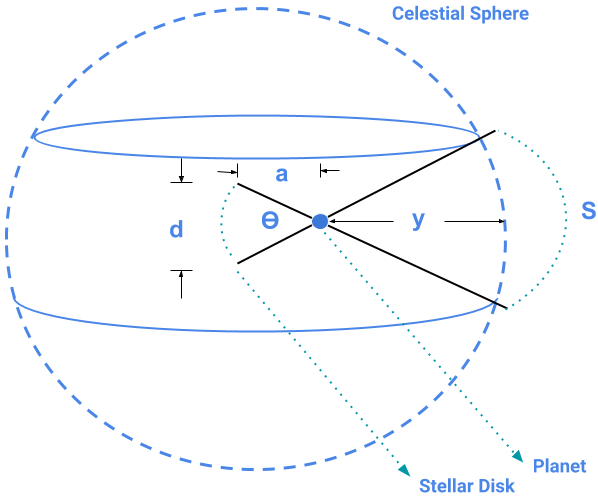
\includegraphics[width = 8cm, height = 7cm]{./Graficos/Capitulo_2/Illustrations/Prob_1.jpg}} 
\caption{\scriptsize{Geometry of the region swept out by the shadow of the planet during one orbital period on the celestial sphere. The planet is located at a distance $a$ from the parent star, and the stellar disk is assumed to have diameter $d_\star$}. In this particular case, the size of the planet is negligible. The total area swept out is projected onto the celestial sphere as represented by the strip cover by the angle $S$. The figure is inspired by \cauthor{1984Icar...58..121B} (\citeyear{1984Icar...58..121B}) work.}
\label{fig:Transit_1}
\end{figure}

In this case, the transit will not be produced by the point-like source but by its rings as a whole. This results in dips in the stellar flux revealing key system parameters. The geometry for this scenario is shown in \autoref{fig:Transit_2} where $R_\star$ is the stellar disk radius, $a$ represents the orbital semi-major axis and $R_H$ is the Hill sphere radius. The orbital inclination of $i = 0^\circ$ means the pole is on, whilst $i = 90^\circ$ means the equator is on. The transit can occur in two different ways:\\

\begin{enumerate}
\item Grazing transit $\textnormal{a} \cos \textnormal{i} \leq \textnormal{R}_\star + \textnormal{R}_\textnormal{H}$
\item Full transit $\textnormal{a} \cos \textnormal{i} \leq \textnormal{R}_\star - \textnormal{R}_\textnormal{H}$
\end{enumerate}

\begin{figure}[!ht]
\centering
  \subfloat{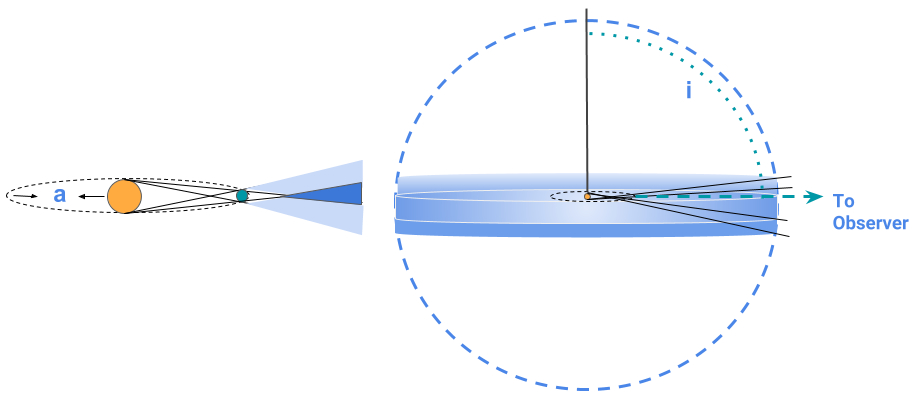
\includegraphics[width = 14cm, height = 6.2cm]{./Graficos/Capitulo_2/Illustrations/Prob_2.jpg}} 
\caption{\scriptsize{Geometry of the region swept out by the shadow of the planet during one orbital period on the celestial sphere. Though the planet is considered to have a negligible size, the Hill sphere where the rings are contained has a non-zero radius. The area swept out on the celestial sphere accounts for the inclination angle of the planet as seen by an observer located on the Earth. The figure is inspired by \cauthor{Cameron2016} (\citeyear{Cameron2016}) work.}}
\label{fig:Transit_2}
\end{figure}

In the absence of any prior knowledge of the system's inclination, the probability of transits being visible over interstellar distances is given by the fraction of the celestial sphere swept out by the planet's shadow as is shown in \autoref{fig:Transit_2} \cauthor{Cameron2016} (\citeyear{Cameron2016}). This is mainly dominated by the orbital inclination of the planet. Considering that the angle between the orbital inclination pole and the line of sight lies in a range ($i$, $i + \Delta i$), and it is randomly distributed as was assumed before, and also that transits occur only in nearly edge-on orbits i.e. $\textnormal{a} \cos \textnormal{i} \leq \textnormal{R}_\star + \textnormal{R}_\textnormal{H}$, we expect the probability to be uniform in $\mathrm{\cos \textnormal{i}}$ as shown in \autoref{fig:Transit_3}. Thus, the transit probability for randomly oriented orbits will be given by

\begingroup
\Large
\begin{equation}
\textnormal{P} \left( \cos \textnormal{i} < \frac{\textnormal{R}_\star + \textnormal{R}_\textnormal{H}}{\textnormal{a}} \right) = \frac{\textnormal{R}_\star + \textnormal{R}_\textnormal{H}}{\textnormal{a}}
 \label{eq:ProbTransit_4}
\end{equation}
\endgroup

\begin{figure}[!ht]
\centering
  \subfloat{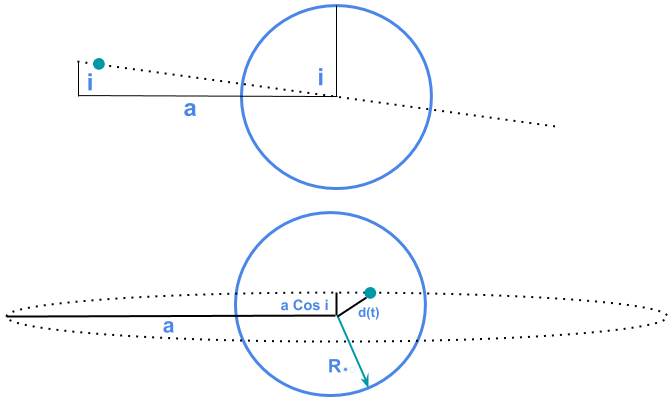
\includegraphics[width = 12cm, height = 7.3cm]{./Graficos/Capitulo_2/Illustrations/Prob_4.jpg}} 
\caption{\scriptsize{Geometry of the transit accounting for the inclination of the orbit. If $\textnormal{a} \cos \textnormal{i} \leq \textnormal{R}_\star + \textnormal{R}_\textnormal{H}$ the transit is grazing, while if $\textnormal{a} \cos \textnormal{i} \leq \textnormal{R}_\star - \textnormal{R}_\textnormal{H}$ the transit is full. As a random orientation of the orbit is considered the probability is uniform in ($\cos \textnormal{i}$) and reduces to the results shown in \autoref{eq:ProbTransit_4}}}
\label{fig:Transit_3}
\end{figure}

Then, in short, the transit probability of exoplanetary-rings in orbit around a given star where the orbital inclination is randomly distributed will be set by \autoref{eq:ProbTransit_4}, where we only need to consider the stellar and planet Hill sphere radii $R_\star$ and $R_H$ respectively, and the orbital semi-major axis. Apart from this, we need to care about when, and how long the rings can co-exist inside the Hill sphere of the planet. This probability was added at the end in order to study the overall change of what was assumed in \autoref{eq:Probabilities} and is presented in the next sub-section. 

\subsection{Rings Lifetime} \label{subsec:RingsSec}

It is well-known that the rings formation is a nonstatic phenomenon, and there is no privileged epoch in the formation of a planetary system when these features can form. On the other hand the only example, so far, we have to compare with, is our own solar system, making the statistical comparison quite hard in terms of deriving the exact formation conditions and time ranges. Nevertheless, simulations and current observations allow us to estimate the main processes that modify these structures, and give us a glimpse on their formation timescales.\\

Currently, most of the statistics are based on \textit{Hot Jupiters} \cauthor{2013pss3.book..309T} (\citeyear{2013pss3.book..309T}). However, there exist different problems with this, because the formation of rings around such objects can be affected by the low-obliquities causing the rings to edge-on or the small Hill sphere radius where they can be embedded in. In addition, viscous and Poynting-Robertson drags cause particle loss, and the high equilibrium black-body temperatures avoid materials to remain the solid state. Survival of the remnant ring depends on if they were created by tidal disruptions or continuous feeding because this will set the timescale on which the rings are expected to exist \cauthor{1984prin.conf..641H} (\citeyear{1984prin.conf..641H}). In our particular case, the most important question regarding the rings is: What is their age?. We need to know how long they are expected to live in order to properly compute the probability of observing ring systems around a planet given the overall age of the star and the planetary system itself. The age of the rings can be affected by the mean residence time of the particles on the rings or by how long the structure/sources have been in place For example in the case of Jupiter, if some moons suddenly disappear, or cease emitting dust, the rings will dissipate in $\sim 10^5$yr \cauthor{2013pss3.book..309T} (\citeyear{2013pss3.book..309T}). Interaction and physical processes may change or reset the age as can be the shepherding of the moons inside the rings leading to an age range of $100\times 10^6$-$6\times10^8$yr \cauthor{1994P&SS...42.1139C} (\citeyear{1994P&SS...42.1139C}), or ring's viscous spreading ($10^5$-$10^9$yr based on Saturn's ring A) \cauthor{2009sfch.book..537C} (\citeyear{2009sfch.book..537C}) or ($\sim10^9$yr) from viscous timescales if the gas is considered to be non-turbulent \cauthor{1984prin.conf..641H} (\citeyear{1984prin.conf..641H}). There is also a chance that the ring is completely disrupted (based on the fragmentation criteria), so in that case we end up with a timescale for complete loss of the rings of $10^{7}$-$10^8$yr \cauthor{1994P&SS...42.1139C} (\citeyear{1994P&SS...42.1139C}) or based on evolutionary processes $< 10^8$yr \cauthor{2009sfch.book..537C} (\citeyear{2009sfch.book..537C}). On the other hand, considering cometary passages which could break a satellite or to tidally disrupt the comet applied to Saturn's ring lead to a time range of $10^7$-$10^8$yr for the A-ring, $10^8$-$10^9$yr for the B-ring, and $10^7$yr from radial spreading \cauthor{2009sfch.book..537C} (\citeyear{2009sfch.book..537C}).\\

As has been presented above, different age ranges can be derived for the rings lifetime through models and observations of our own solar system. However, the remaining question is: Do they form at the very beginning, in the middle or at the end of the planetary system formation?. According to \cauthor{2009Icar..199..413C} (\citeyear{2009Icar..199..413C}) the main core of Saturn's B-ring was formed in the first Gyr of the solar system in which collisions are expected to be much more likely. However, from simulations it is pointed out Saturn's ring formation can be understood a huge disruption near the end of the planetary formation period during which the circum-planetary gas disk is still present \cauthor{2010Natur.468..943C} (\citeyear{2010Natur.468..943C}). If we look to Uranus or Neptune, possibly they have been less affected and have not changed dramatically over the age of the solar system, where rings and moons have been oscillating between accretion and disruption for many Gyr \cauthor{2013pss3.book..309T} (\citeyear{2013pss3.book..309T}).\\

In general, there is no complete consensus on whether the rings form at the beginning, or at the end of the planetary formation process, neither on the time they can live as a ringed-structure around the planet. Base on this, we decided to introduce a fifth probability to account for the most likely lifespan a ring can have. The probability is defined in \autoref{eq:Prob_5}, but it is necessary to have in mind that as it is hard to guarantee the exact moment in time where they form, then this probability assumes each time interval has the same chance and we can only provide an estimation based on the mean-rings lifespan as a function of the stellar age.  

\begingroup
\Large
\begin{equation}
\textnormal{P}_5 = \frac{\textnormal{Rings}~\textnormal{lifespan}}{\textnormal{Host}~\textnormal{star's}~\textnormal{age}}
 \label{eq:Prob_5}
\end{equation}
\endgroup

%============================================================================================================================================================

\section{Monte-Carlo simulations} \label{sec:MCSec}

As was shown in \autoref{sec:PowerLawSec}, we have two different ways to generate the exoplanetary mass-period distribution either by considering a weak correlation e.g. $\beta$-distribution or using a simple power law derived from the observations. One way or another, we are able to generate a new sample of planets with mass and period following a given distribution using the Monte-Carlo method. This method consists in drawing a sample of $N$ values which follows the wanted distribution using randomly distributed numbers.\\

%In the first case, we have the $\beta$-distribution addressed in \autoref{subsec:BetaDist}. A sample of $10.000$ mass-period pairs were generated following \autoref{eq:Beta_Monte}, where ($\alpha_\textnormal{m}, \beta_\textnormal{m}$), ($\alpha_\textnormal{p}, \beta_\textnormal{p}$), and ($\delta_\textnormal{1}, \delta_\textnormal{2}$) were created using pseudo-random numbers following a $\beta$-distribution as mentioned in \cauthor{1538-3881-134-5-2061} \citeyear{1538-3881-134-5-2061}. The mass and period range covers $0.008 \leq \textnormal{m/Mj} \leq 26.7$, and $0.8079 \leq \textnormal{p/days} \leq 6776.1$ respectively.\\

% \begingroup
% \Large
% \begin{equation}
%   \begin{align*}
%   \textnormal{m}~~&=~~155.5*(\alpha_\textnormal{m} + \delta_\textnormal{1}) / (\alpha_\textnormal{m} + \delta_\textnormal{1} + \beta_\textnormal{m} + \delta_\textnormal{2}) \\[10pt]
%   \textnormal{p}~~&=~~11650.0*(\alpha_\textnormal{p} + \delta_\textnormal{1}) / (\alpha_\textnormal{p} + \delta_\textnormal{1} + \beta_\textnormal{p} + \delta_\textnormal{2})
%  \label{eq:Beta_Monte}
%  \end{align*}
% \end{equation}
% \endgroup \\

%The period/mass, period/semi-major axis, and mass/semi-major axis are shown in figures \autoref{fig:PeriodMass_Beta},\autoref{fig:PeriodMajor_Beta}, and  \autoref{fig:MassMajor_Beta} respectively where each dot corresponds to each pair generated using the $\beta$-distribution method, and the semi-major axis was computed using Kepler's third law.\\ 


% \begin{figure}[!ht]
% \centering
%   \subfloat{\includegraphics[width = 12cm, height = 9cm]{./Graficos/Capitulo_2/2_Exop_distributions/Period_mass_distribution_2.png}} 
% \caption{\scriptsize{Exoplanetary period (days) as a function of exoplanetary mass ($\textnormal{Mj}$). Each value corresponds to a planetary mass-period pair generated following the $\beta$-distribution approach as mentioned in \cauthor{1538-3881-134-5-2061} \citeyear{1538-3881-134-5-2061} using a Monte-Carlo simulation of $10.000$ objects. The majority of planets tend to aggregate around the small period and mass values.}}
% \label{fig:PeriodMass_Beta}
% \end{figure}
% 
% \begin{figure}[!ht]
% \centering
%   \subfloat{\includegraphics[width = 12cm, height = 9cm]{./Graficos/Capitulo_2/2_Exop_distributions/Period_major_distribution_2.png}} 
% \caption{\scriptsize{Exoplanetary period (days) as a function of semi-major axis ($\textnormal{AU}$). Each value corresponds to a planetary mass-period pair generated following the $\beta$-distribution approach as mentioned in \cauthor{1538-3881-134-5-2061} \citeyear{1538-3881-134-5-2061} using a Monte-Carlo simulation of $10.000$ objects. The semi-major axis was derived using Kepler's third law which sets the left-and right boundaries of the distribution. Planets beyond $\textnormal{a} \approx 20 \textnormal{AU}$ cannot be generated due to the period-mass ranges evaluated.}}
% \label{fig:PeriodMajor_Beta}
% \end{figure}
% 
% \begin{figure}[!ht]
% \centering
%   \subfloat{\includegraphics[width = 12cm, height = 9cm]{./Graficos/Capitulo_2/2_Exop_distributions/Mass_major_distribution_2.png}} 
% \caption{\scriptsize{Exoplanetary mass ($\textnormal{Mj}$) as a function of semi-major axis ($\textnormal{AU}$). Each value corresponds to a planetary mass-period pair generated following the $\beta$-distribution approach as mentioned in \cauthor{1538-3881-134-5-2061} \citeyear{1538-3881-134-5-2061} using a Monte-Carlo simulation of $10.000$ objects. The semi-major axis was derived using Kepler's third law which sets the left-and right boundaries of the distribution. Planets beyond $\textnormal{a} \approx 20 \textnormal{AU}$ cannot be generated due to the period-mass ranges evaluated.}}
% \label{fig:MassMajor_Beta}
% \end{figure}

We decided to use the single power law approach as suggested by (\cauthor{2008PASP..120..531C} \citeyear{2008PASP..120..531C}; \cauthor{2006ApJ...646..505B} \citeyear{2006ApJ...646..505B}) to generate the mass-period distribution for exoplanets, and also following the well-known Salpeter- and-Kroupa's power law to generate the stellar masses as was explained in \autoref{subsec:Salpeter} and \autoref{subsec:Kroupa} individually. Following this method, we set the values for the exponents in the case of the exoplanets to $1.16$ and $0.74$ for the mass and the period respectively as suggested in \cauthor{2010EAS....41..107N} (\citeyear{2010EAS....41..107N}) who basically based his results on different observations and corrections to values previously obtained by \cauthor{2008PASP..120..531C} (\citeyear{2008PASP..120..531C}) and \cauthor{2006ApJ...646..505B} (\citeyear{2006ApJ...646..505B}). According to the last, we can generate a sample of exoplanetary masses and periods in a range covering $0.3 \leq \textnormal{m/Mj} \leq 10$, and $2 \leq \textnormal{p/days} \leq 2000$. Thus, a sample of $10.000$ pairs was drew following the method explained in \autoref{sec:PowerLawSec}. In \autoref{fig:Mass_Nielsen} and \autoref{fig:Period_Nielsen} the histogram and the cumulative function for the generated values are shown in blue whilst the orange dashed line shows the expected shape that these values should follow from the original power law. The figures on the left are shown in linear scale while those on the right are in logarithmic scale. It is clear that both, the mass and period values simulated follow the original power law. Same process was performed using the $\beta$-distribution but the final results were not so different. For comparison the period/mass, period/semi-major axis, and mass/semi-major axis are shown in figures \autoref{fig:PeriodMass_Nielsen},\autoref{fig:PeriodMajor_Nielsen}, and  \autoref{fig:MassMajor_Nielsen} respectively. However, as using the power law we can double check that the simulated values follow the original trend, which is not the case for the $\beta$-distribution where the constants are imposed from their observations, we decided use the power-law method to generate our final sample of mass-period pairs.\\ 

\begin{figure}[!ht]
\centering
  \subfloat{\includegraphics[width = 18.5cm, height = 15.5cm, scale = 1.0, angle = 90]{./Graficos/Capitulo_2/2_Exop_distributions/Mass_distribution_Nielsen.png}} 
\caption{\scriptsize{Monte-Carlo simulation of exoplanetary mass distribution following a power law of slope $1.16$ \cauthor{2010EAS....41..107N} (\citeyear{2010EAS....41..107N}). \textit{\textbf{Top-Left}}: histogram corresponding to the $10.000$ masses generated using the Monte-Carlo approach. The orange line represents the analytic shape the distribution should follow. \textit{\textbf{Top-Right}}: same as figure described in \textit{Top-Left} but using logarithmic x-scale for comparison. \textit{\textbf{Bottom-Left}}: cumulative mass distribution function for the generated masses is shown in blue while the analytic is shown in orange. \textit{\textbf{Bottom-Right}}: same as described in \textit{Bottom-Left} but using logarithmic-scales. The feature produced at low mass values which makes both curves differ because the minimum simulated value is slightly above the possible minimum mass.%The feature produced at low mass values which makes both curves differ is an artifact of the logarithmic-scale and it does not correspond to a real deviation in the simulated data.
}}
\label{fig:Mass_Nielsen}
\end{figure}

\begin{figure}[!ht]
\centering
  \subfloat{\includegraphics[width = 18.5cm, height = 15.5cm, scale = 1.0, angle = 90]{./Graficos/Capitulo_2/2_Exop_distributions/Period_distribution_Nielsen.png}} 
\caption{\scriptsize{Monte-Carlo simulation of exoplanetary period distribution following a power law of slope $0.74$ \cauthor{2010EAS....41..107N} (\citeyear{2010EAS....41..107N}). \textit{\textbf{Top-Left}}: histogram corresponding to the $10.000$ periods generated using the Monte-Carlo approach. The orange line represents the analytic shape the distribution should follow. \textit{Top-Right}: same as figure described in \textit{Top-Left} but using logarithmic x-scale for comparison. \textit{\textbf{Bottom-Left}}: cumulative mass distribution function for the generated masses is shown in blue while the analytic is shown in orange. \textit{\textbf{Bottom-Right}}: same as described in \textit{\textbf{Bottom-Left}} but using logarithmic-scales. The feature produced at low mass values which makes both curves differ because the minimum simulated value is slightly above the possible minimum mass.%The feature produced at low mass values which makes both curves differ is an artifact of the logarithmic-scale and it does not correspond to a real deviation in the simulated data.
}}
\label{fig:Period_Nielsen}
\end{figure}

\begin{figure}[!ht]
\centering
  \subfloat{\includegraphics[width = 12cm, height = 9cm]{./Graficos/Capitulo_2/2_Exop_distributions/Period_mass_distribution.png}} 
\caption{\scriptsize{Exoplanetary period (days) as a function of exoplanetary mass ($\textnormal{Mj}$). Each value corresponds to a planetary mass-period pair generated following power-law distribution approach as mentioned in \cauthor{2010EAS....41..107N} (\citeyear{2010EAS....41..107N}) using a Monte-Carlo simulation of $10.000$ objects. The majority of planets tend to aggregate around the small period and mass values. %In comparison to \autoref{fig:PeriodMass_Beta}, the period-range is smaller, but the general trend is kept.
}}
\label{fig:PeriodMass_Nielsen}
\end{figure}

\begin{figure}[!ht]
\centering
  \subfloat{\includegraphics[width = 12cm, height = 9cm]{./Graficos/Capitulo_2/2_Exop_distributions/Period_major_distribution.png}} 
\caption{\scriptsize{Exoplanetary period (days) as a function of semi-major axis ($\textnormal{AU}$). Each value corresponds to a planetary mass-period pair generated following power-law distribution approach as mentioned in \cauthor{2010EAS....41..107N} (\citeyear{2010EAS....41..107N}) using a Monte-Carlo simulation of $10.000$ objects. The semi-major axis was derived using Kepler's third law which sets the left-and right boundaries of the distribution. %In comparison to \autoref{fig:PeriodMajor_Beta}, planets beyond $\textnormal{a} \approx 7 \textnormal{AU}$ cannot be generated due to the period-mass ranges evaluated.
}}
\label{fig:PeriodMajor_Nielsen}
\end{figure}

\begin{figure}[!ht]
\centering
  \subfloat{\includegraphics[width = 12cm, height = 9cm]{./Graficos/Capitulo_2/2_Exop_distributions/Mass_major_distribution.png}} 
\caption{\scriptsize{Exoplanetary mass ($\textnormal{Mj}$) as a function of semi-major axis ($\textnormal{AU}$). Each value corresponds to a planetary mass-period pair generated power-law distribution approach as mentioned in \cauthor{2010EAS....41..107N} (\citeyear{2010EAS....41..107N}) using a Monte-Carlo simulation of $10.000$ objects. The semi-major axis was derived using Kepler's third law which sets the left-and right boundaries of the distribution. %In comparison to \autoref{fig:MassMajor_Beta}, planets beyond $\textnormal{a} \approx 7 \textnormal{AU}$ cannot be generated due to the period-mass ranges evaluated.
}}
\label{fig:MassMajor_Nielsen}
\end{figure}

Finally, the same power-law method was used to generate the stellar mass. As was introduced in \autoref{subsec:Salpeter} and \autoref{subsec:Kroupa}, we have two different power laws which can describe the stellar mass functions. Taking into account that in general there is no consensus on a single exponent which could describe the distribution of stellar masses in the universe, we decided to test both exponents but paying more attention to the Kroupa's initial mass function distribution because we think it is a more realistic description of the stellar IMF. Following this, we created once again a sample of $10.000$ stars following the initial mass function described by a Salpeter's and Kroupa's exponent. In the case of Salpeter, the mass range covers  $0.1 \leq \textnormal{m/M$_\odot$} \leq 10$ with an exponent of $2.35$, whilst the Kroupa's range covers $0.1 \leq \textnormal{m/M$_\odot$} \leq 0.5$ with an exponent of $1.3$, and an exponent of $2.3$ for $0.5 \leq \textnormal{m/M$_\odot$} \leq 10$. The drawn distributions are shown in \autoref{fig:Salpeter_IMF} and \autoref{fig:Kroupa_IMF}, where the histogram and cumulative functions are shown in blue and the original power law distributions are shown with the dashed orange line. In the case of the Kroupa's distribution, a fine break can be seen in the logarithmic scale figure for the small stellar masses due to the fact that we are using two different exponents for different mass ranges.\\  

\begin{figure}[!ht]
\centering
  \subfloat{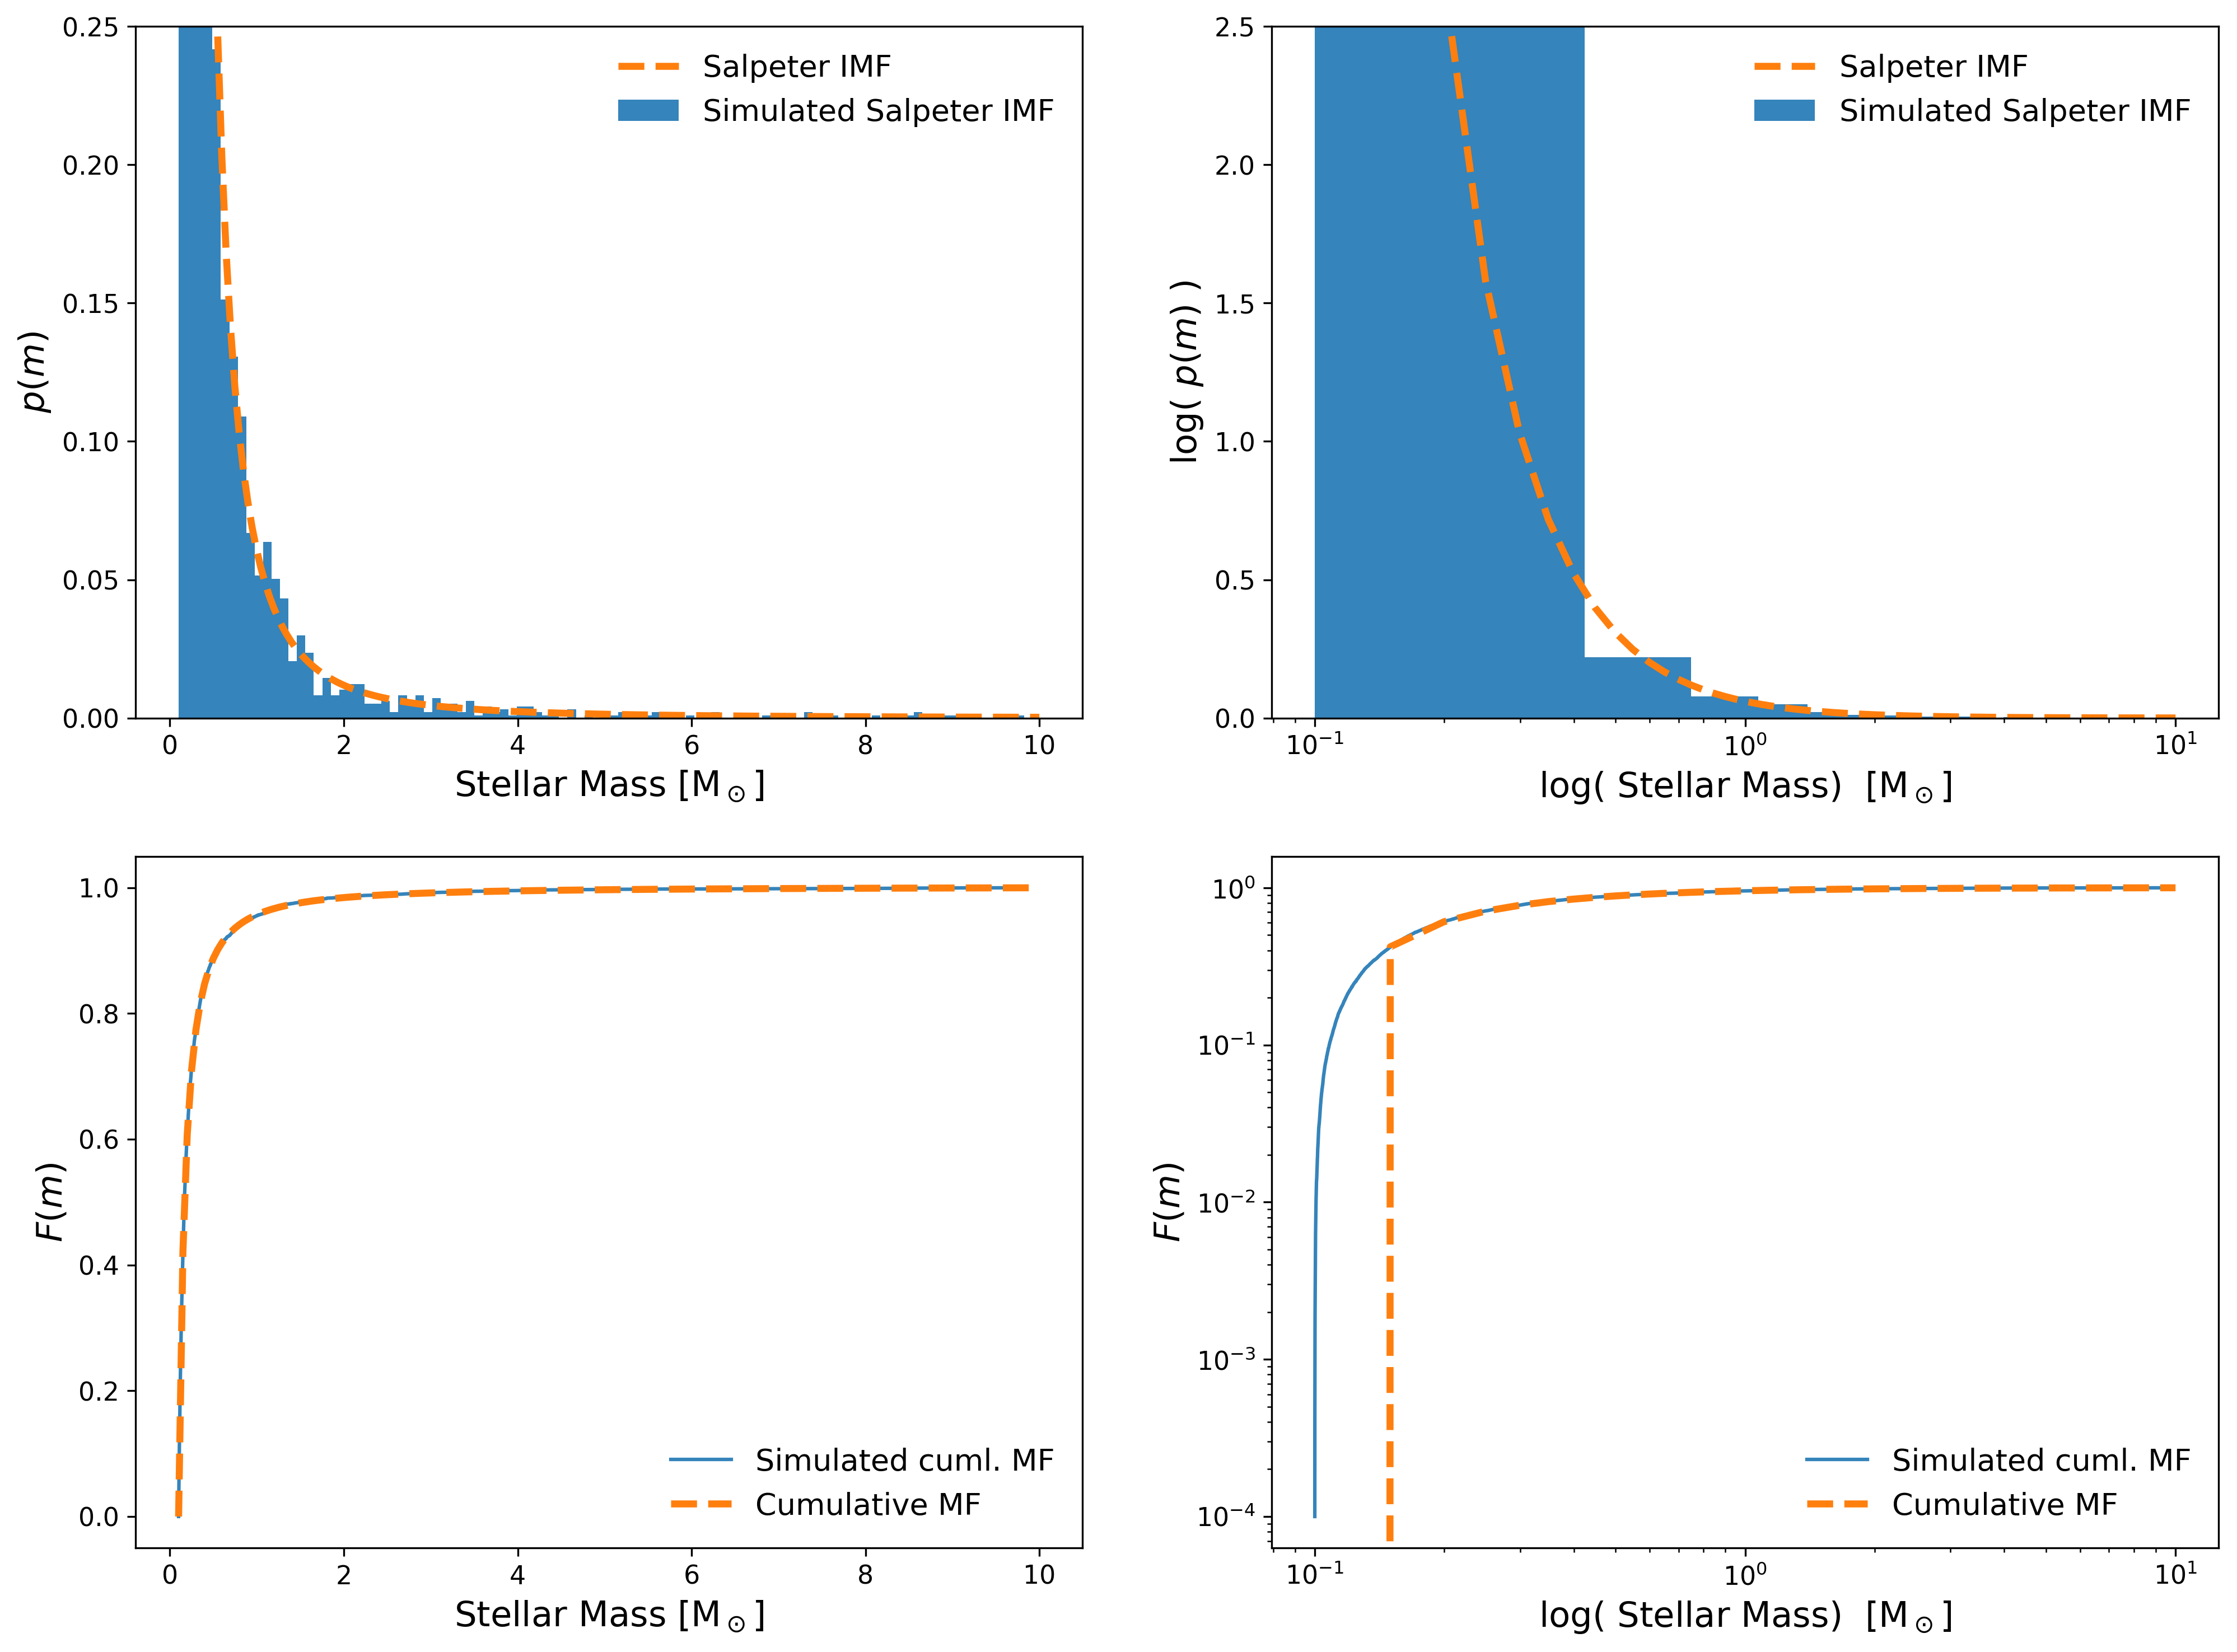
\includegraphics[width = 18.5cm, height = 15.5cm, scale = 1.0, angle = 90]{./Graficos/Capitulo_2/2_Exop_distributions/Salpeter.png}} 
\caption{\scriptsize{Monte-Carlo simulation of stellar mass distribution following a Salpeter's power law. \textit{\textbf{Top-Left}}: histogram corresponding to the $10.000$ stellar masses generated using the Monte-Carlo approach. The orange line represents the analytic shape the distribution should follow. \textit{\textbf{Top-Right}}: same as figure described in \textit{Top-Left} but using logarithmic x-scale for comparison. \textit{\textbf{Bottom-Left}}: cumulative stellar mass distribution function for the generated masses is shown in blue while the analytic is shown in orange. \textit{Bottom-Right}: same as described in \textit{\textbf{Bottom-Left}} but using logarithmic-scales. The feature produced at low mass values which makes both curves differ because the minimum simulated date is slightly above the possible minimum mass.%The feature produced at low mass values which makes both curves differ is an artifact of the logarithmic-scale and it does not correspond to a real deviation in the simulated data.
}}
\label{fig:Salpeter_IMF}
\end{figure}

\begin{figure}[!ht]
\centering
  \subfloat{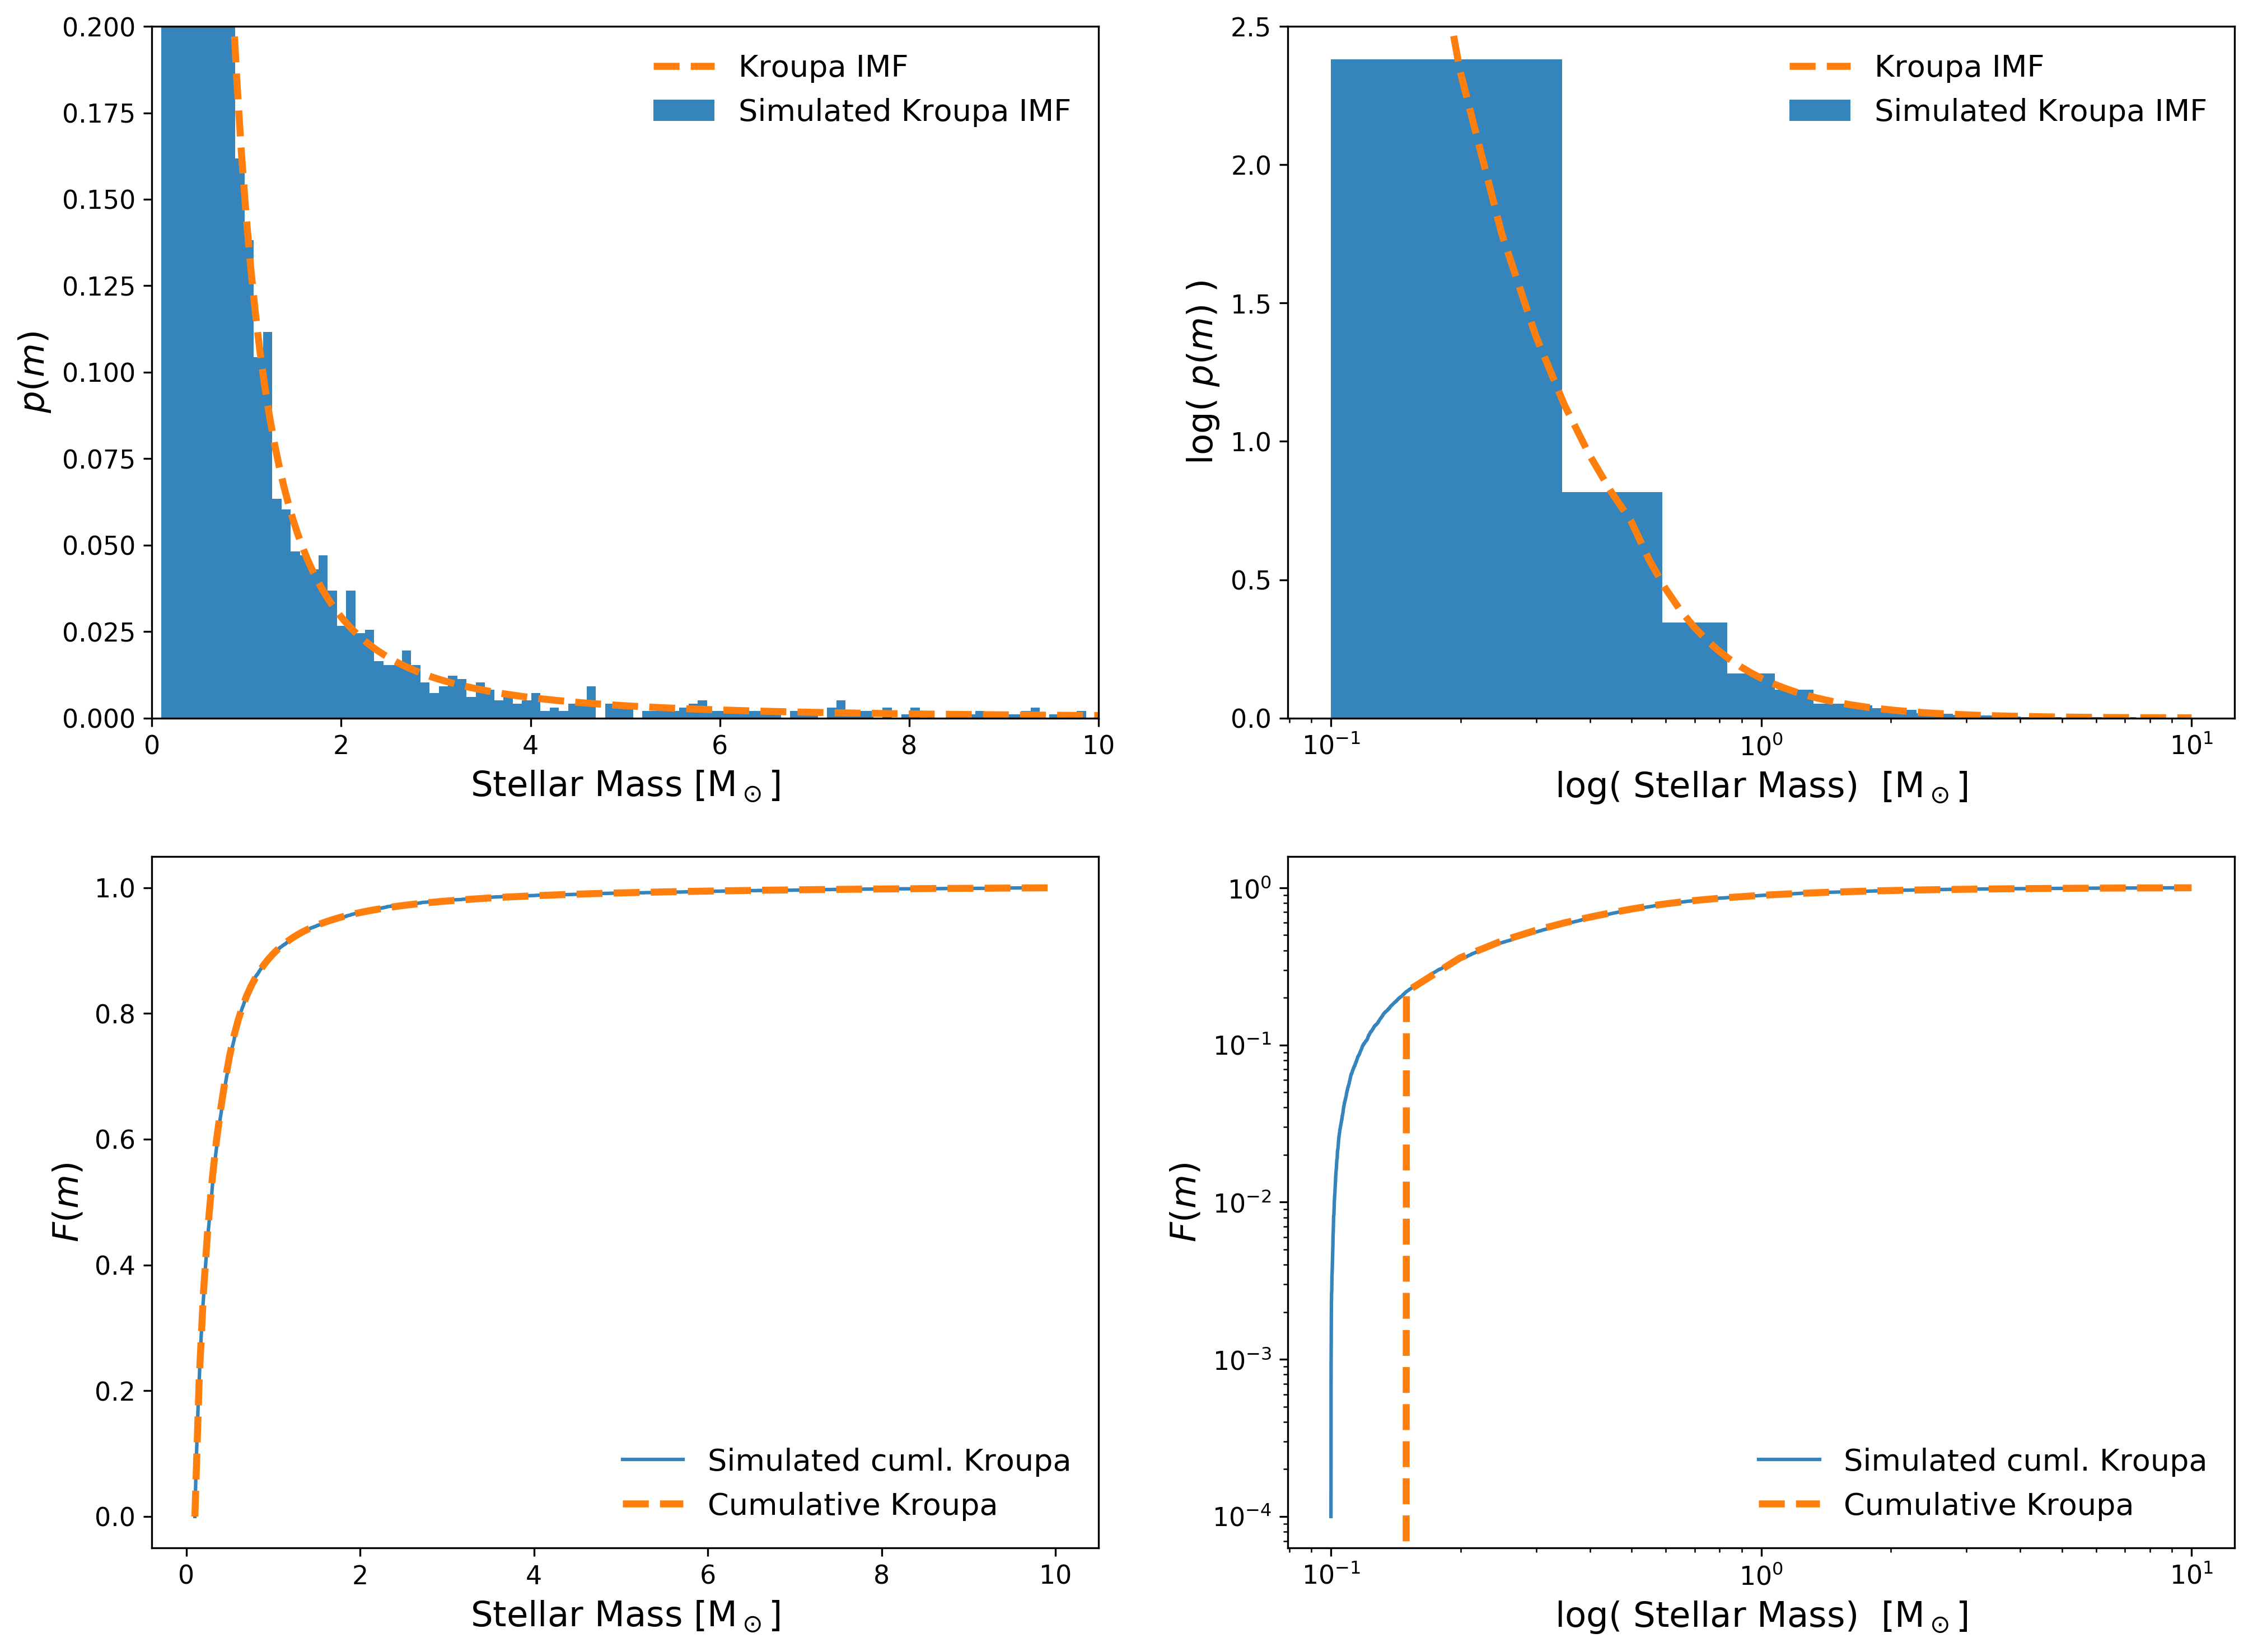
\includegraphics[width = 18.5cm, height = 15.5cm, scale = 1.0, angle = 90]{./Graficos/Capitulo_2/2_Exop_distributions/Kroupa.png}} 
\caption{\scriptsize{Monte-Carlo simulation of stellar mass distribution following a Kroupa's power law. \textit{\textbf{Top-Left}}: histogram corresponding to the $10.000$ stellar masses generated using the Monte-Carlo approach. The orange line represents the analytic shape the distribution should follow. \textit{\textbf{Top-Right}}: same as figure described in \textit{Top-Left} but using logarithmic x-scale for comparison. \textit{\textbf{Bottom-Left}}: cumulative stellar mass distribution function for the generated masses is shown in blue while the analytic is shown in orange. \textit{Bottom-Right}: same as described in \textit{\textbf{Bottom-Left}} but using logarithmic-scales. The feature produced at low mass values which makes both curves differ because the minimum simulated date is slightly above the possible minimum mass.%The feature produced at low mass values which makes both curves differ is an artifact of the logarithmic-scale and it does not correspond to a real deviation in the simulated data.
}}
\label{fig:Kroupa_IMF}
\end{figure}

Summarizing, we generated a sample of $10.000$ exoplanetary mass-period pairs and stellar masses individually following in the case of the exoplanets $\beta$-distribution or a simple power law, and in the case of the stellar initial mass function using two different power laws known as Salpeter's and Kroupa's initial mass function. As we have different ways to generate mock samples, we decided to stick to the power law generation in the case of the exoplanetary mass-period distribution because we are able to check the cumulative function and check if the currently drawn pairs follow the original distributions. In the same way, for the stellar mass generation, we decided to use the Kroupa's distribution because is more general. Having said this, we proceed to use these values and the previous information presented in the last sections to compute the probability of transit detection. This is thoroughly explained in \autoref{sec:AnalyticForm} in which we address this calculation in two different ways. Firstly, using the results from the Monte-Carlo simulations, and secondly evaluating directly the analytic form of the transit probability.     


%============================================================================================================================================================

\section{Detection Probability: Monte-Carlo vs Analytic Form} \label{sec:AnalyticForm}
%============================================================================================================================================================

In \autoref{sec:DetectionProbability}, the main components of the probability of a ringed-system transiting in front of its parent star was addressed. However, the main goal is to constrain for the different exoplanetary mass-period pairs, how this probability changes as a function of the stellar mass. We decided to tackle down this problem in two different ways: i) using the Monte-Carlo results for the exoplanetary mass-period distributions, and ii) simply generating the probability from the analytic form without recurring to any Monte-Carlo generation of values. In both cases, we use the probability function shown in \autoref{eq:FinalDetectProb} which does not include the fifth probability corresponding to the planetary rings' lifetime. This will be addressed separately at the end of this section.\\

First of all, in the case of the Monte-Carlo process, a sample of $10.000$ stars between $0.1 \leq \textnormal{m/M$_\odot$} \leq 10.0$ was generated following the Kroupa's initial mass function. Moreover, a sample of $10.000$ mass-period pairs was also generated following the power law distribution suggested by \cauthor{2010EAS....41..107N} (\citeyear{2010EAS....41..107N}) and explained in \autoref{sec:MCSec}. Once we have set the final sample of exoplanets and stars to be tested, we proceed to evaluate out the detection probability function which is given by \autoref{eq:FinalDetectProb}. It is important to have in mind that in this equation the values corresponding to the exoplanetary mass and period are taken from the Monte-Carlo simulation. Also, the semi-major axis is obtained using Kepler's third law, and the stellar mass is obtained with the Monte-Carlo generation as well. We need to have a relationship between the stellar masses and stellar radii. To achieve this goal, we used two different approaches. The first one assumes that the stars are in the main sequence and follow the regular relation given by $\textnormal{R} \propto \textnormal{M}^{0.8}$. However, this assumes that the stars are already in the ZAMS, have the solar metallicity and are massive stars burning H to He via the CNO chain. This not entirely true for our purposes because we aim to study young stellar populations. Thus, we decided to use the \textit{MESA}-code provided through the \textit{MIST}-package (\cauthor{2016ApJS..222....8D} \citeyear{2016ApJS..222....8D}; \cauthor{2016ApJ...823..102C} \citeyear{2016ApJ...823..102C}) to compute the stellar isochrone for a $20Myr$ star varying the masses between $0.1 \leq \textnormal{m/M$_\odot$} \leq 10.0$ which is the range we are interested in. In \autoref{fig:RMInterpol}, the stellar radius versus the stellar mass obtained using the $20Myr$ isochrone is shown. The blue dots correspond to the values retrieved by the model while the orange dots represent a linear interpolation performed to complete some empty regions in the isochrone. Once this is settled, we can assign the expected stellar radius for a given mass assuming that the stellar age is close to $20Myr$.\\ 

\begingroup
\large
\begin{equation}
  \textnormal{Detection Probability} = 0.17 \left(\frac{\textnormal{R}_\star + \textnormal{R}_\textnormal{H}}{\textnormal{a}} \right) \left[ 1 - \left( \frac{\textnormal{Gaia}~\textnormal{Duration} - \textnormal{Eclipse}~\textnormal{Duration}}{\textnormal{Gaia}~\textnormal{Duration}} \right)^\textnormal{n} \right]
 \label{eq:FinalDetectProb}
\end{equation}
\endgroup \\

\begin{figure}[!ht]
\centering
  \subfloat{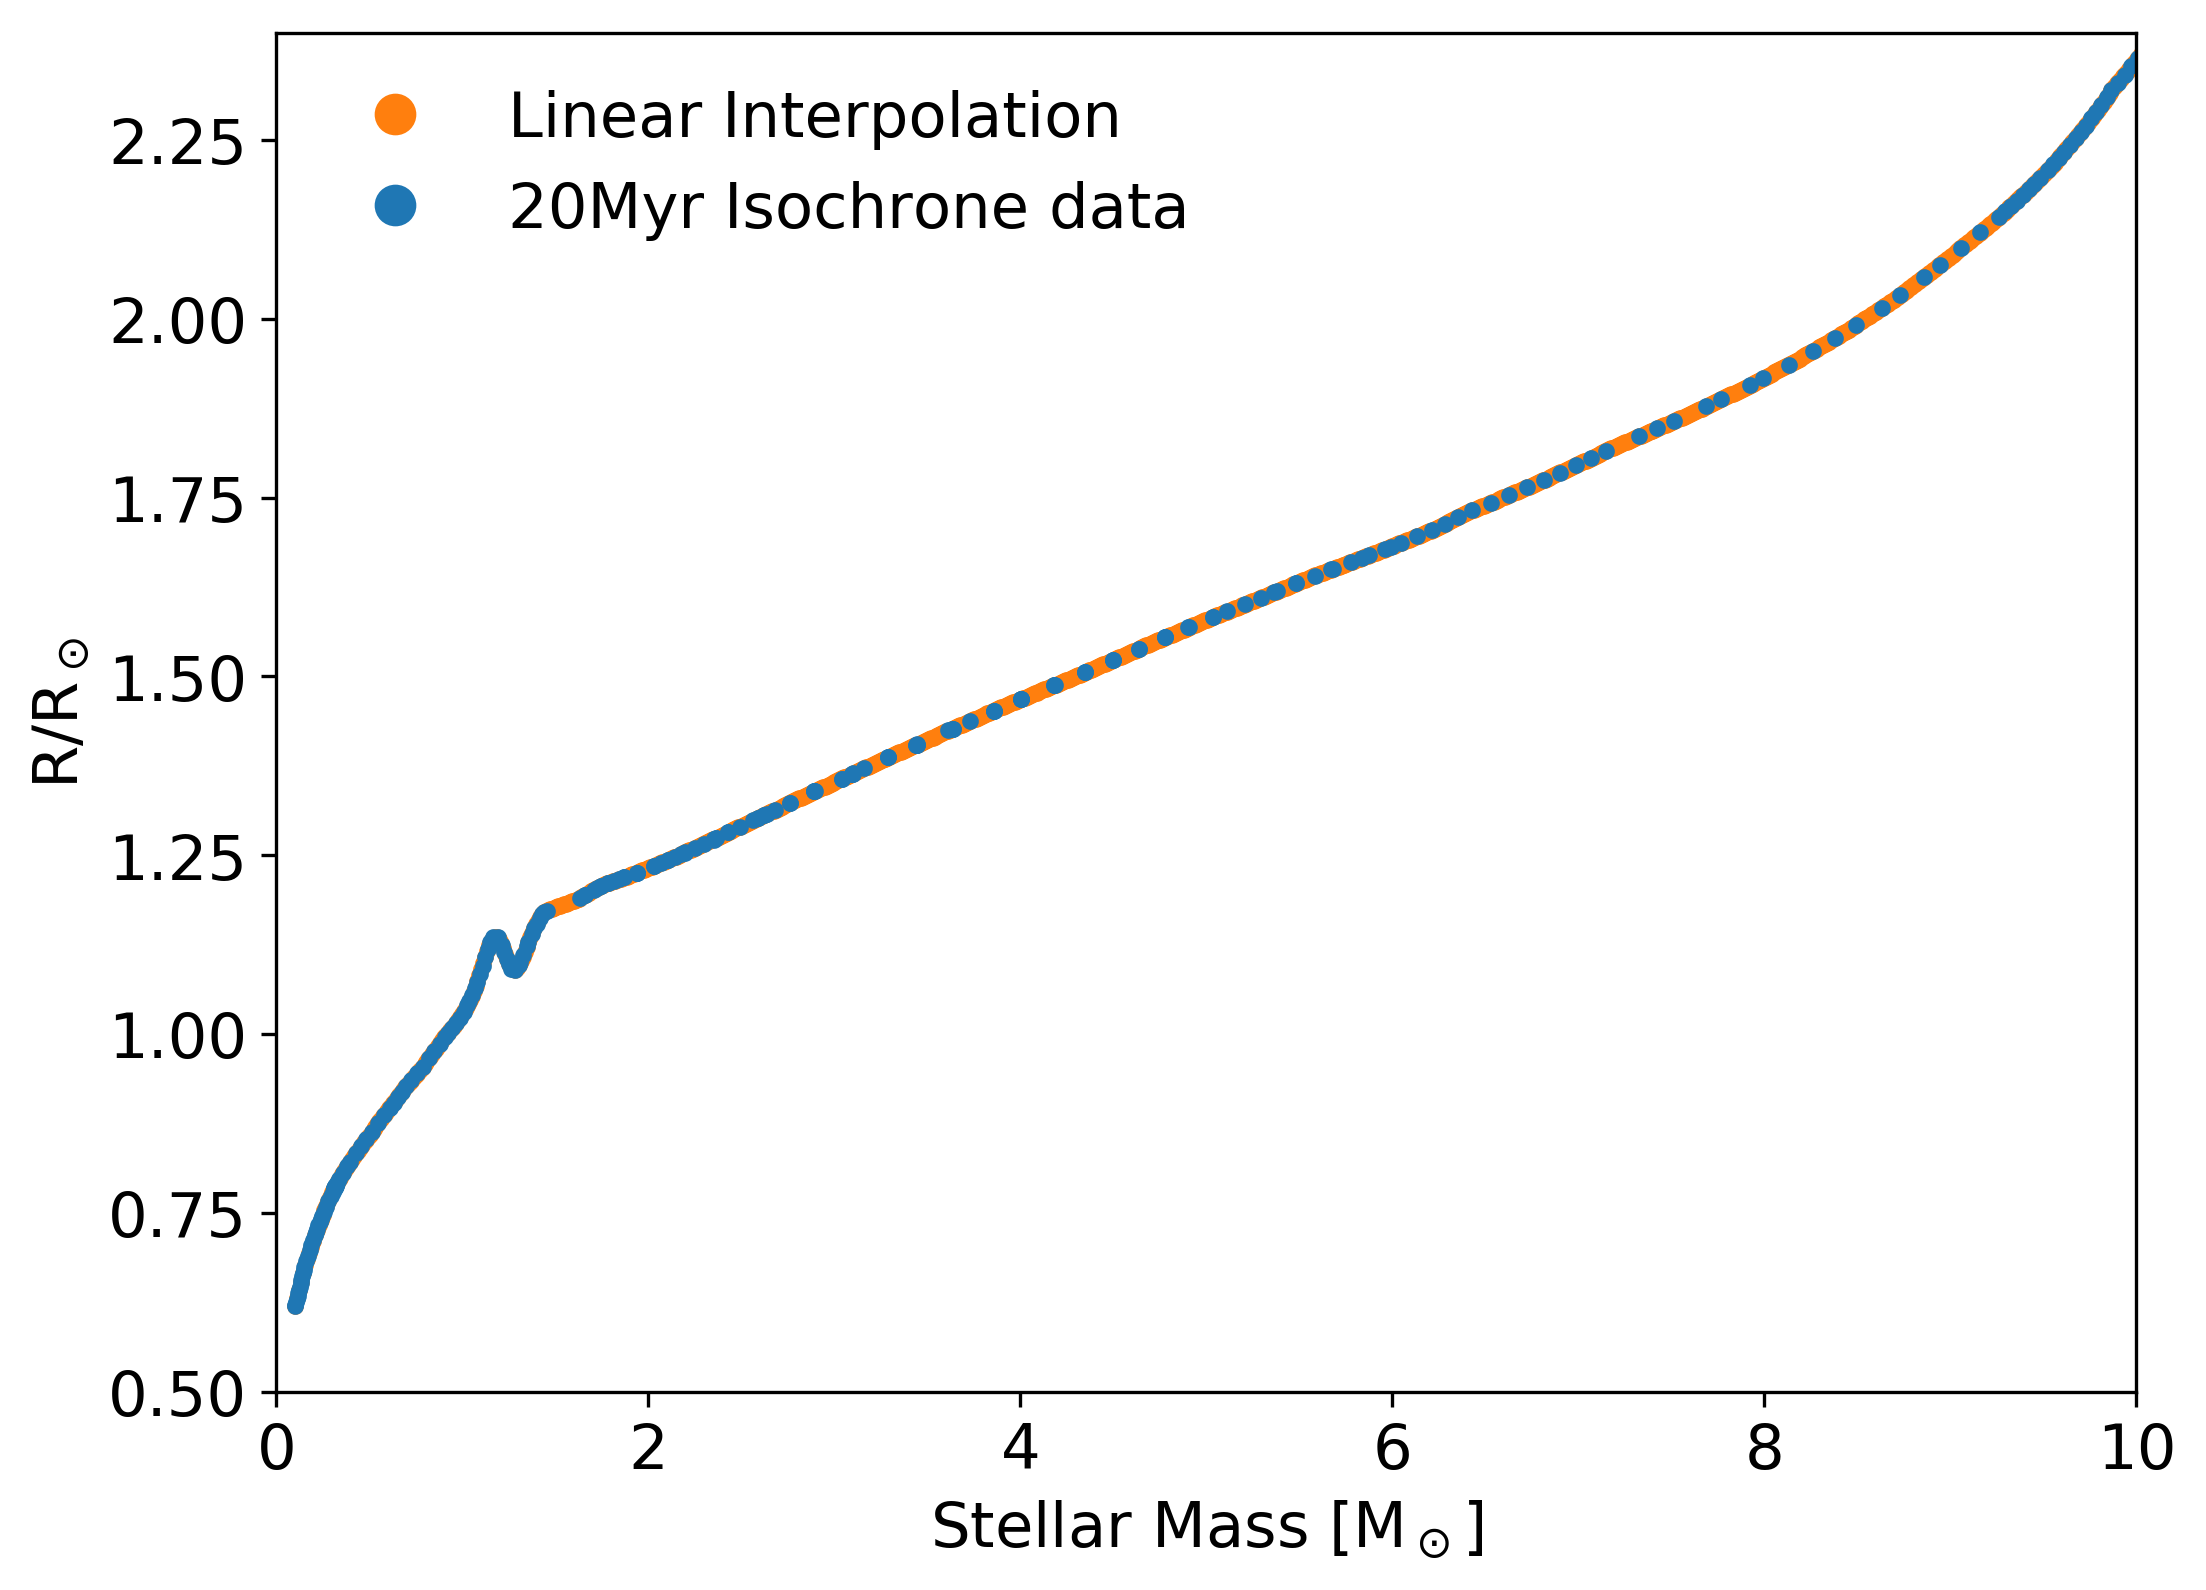
\includegraphics[width = 12cm, height = 9cm]{./Graficos/Capitulo_2/2_Exop_distributions/Linear_Interpolation.png}} 
\caption{\scriptsize{Linear interpolation of a $20 \textnormal{Myr}$ isochrone stellar radius as a function of mass. The blue dots correspond to the stellar radius as a function of stellar mass for a $20 \textnormal{Myr}$ isochrone calculated using the \textit{MIST}-package (\cauthor{2016ApJS..222....8D} \citeyear{2016ApJS..222....8D}; \cauthor{2016ApJ...823..102C} \citeyear{2016ApJ...823..102C}). The orange dots are the result of the linear interpolation performed to fill the gaps in the computed isochrone to properly compare the stellar radius and stellar mass of possible young candidates without assuming standard main-sequence relations but more suitable, real values for our stellar population.}}
\label{fig:RMInterpol}
\end{figure}

Once the function is evaluated using all the different parameters described above, we end up with a detection probability distribution for each exoplanet as a function of the stellar mass as shown in \autoref{fig:MonteKroupaNielsen}. Panel (a) shows the detection probability (occurrence) as a function of stellar mass computed through \autoref{eq:FinalDetectProb} for five randomly selected values out of the $10.000$ simulated. Panel (b) shows exactly the same parameters but in this case, the detection probability was summed up in bins of $0.5M_\odot$ to obtain the total number of detections expected.\\ 

\begin{figure}[!ht]%
    \centering
    \subfloat[]{{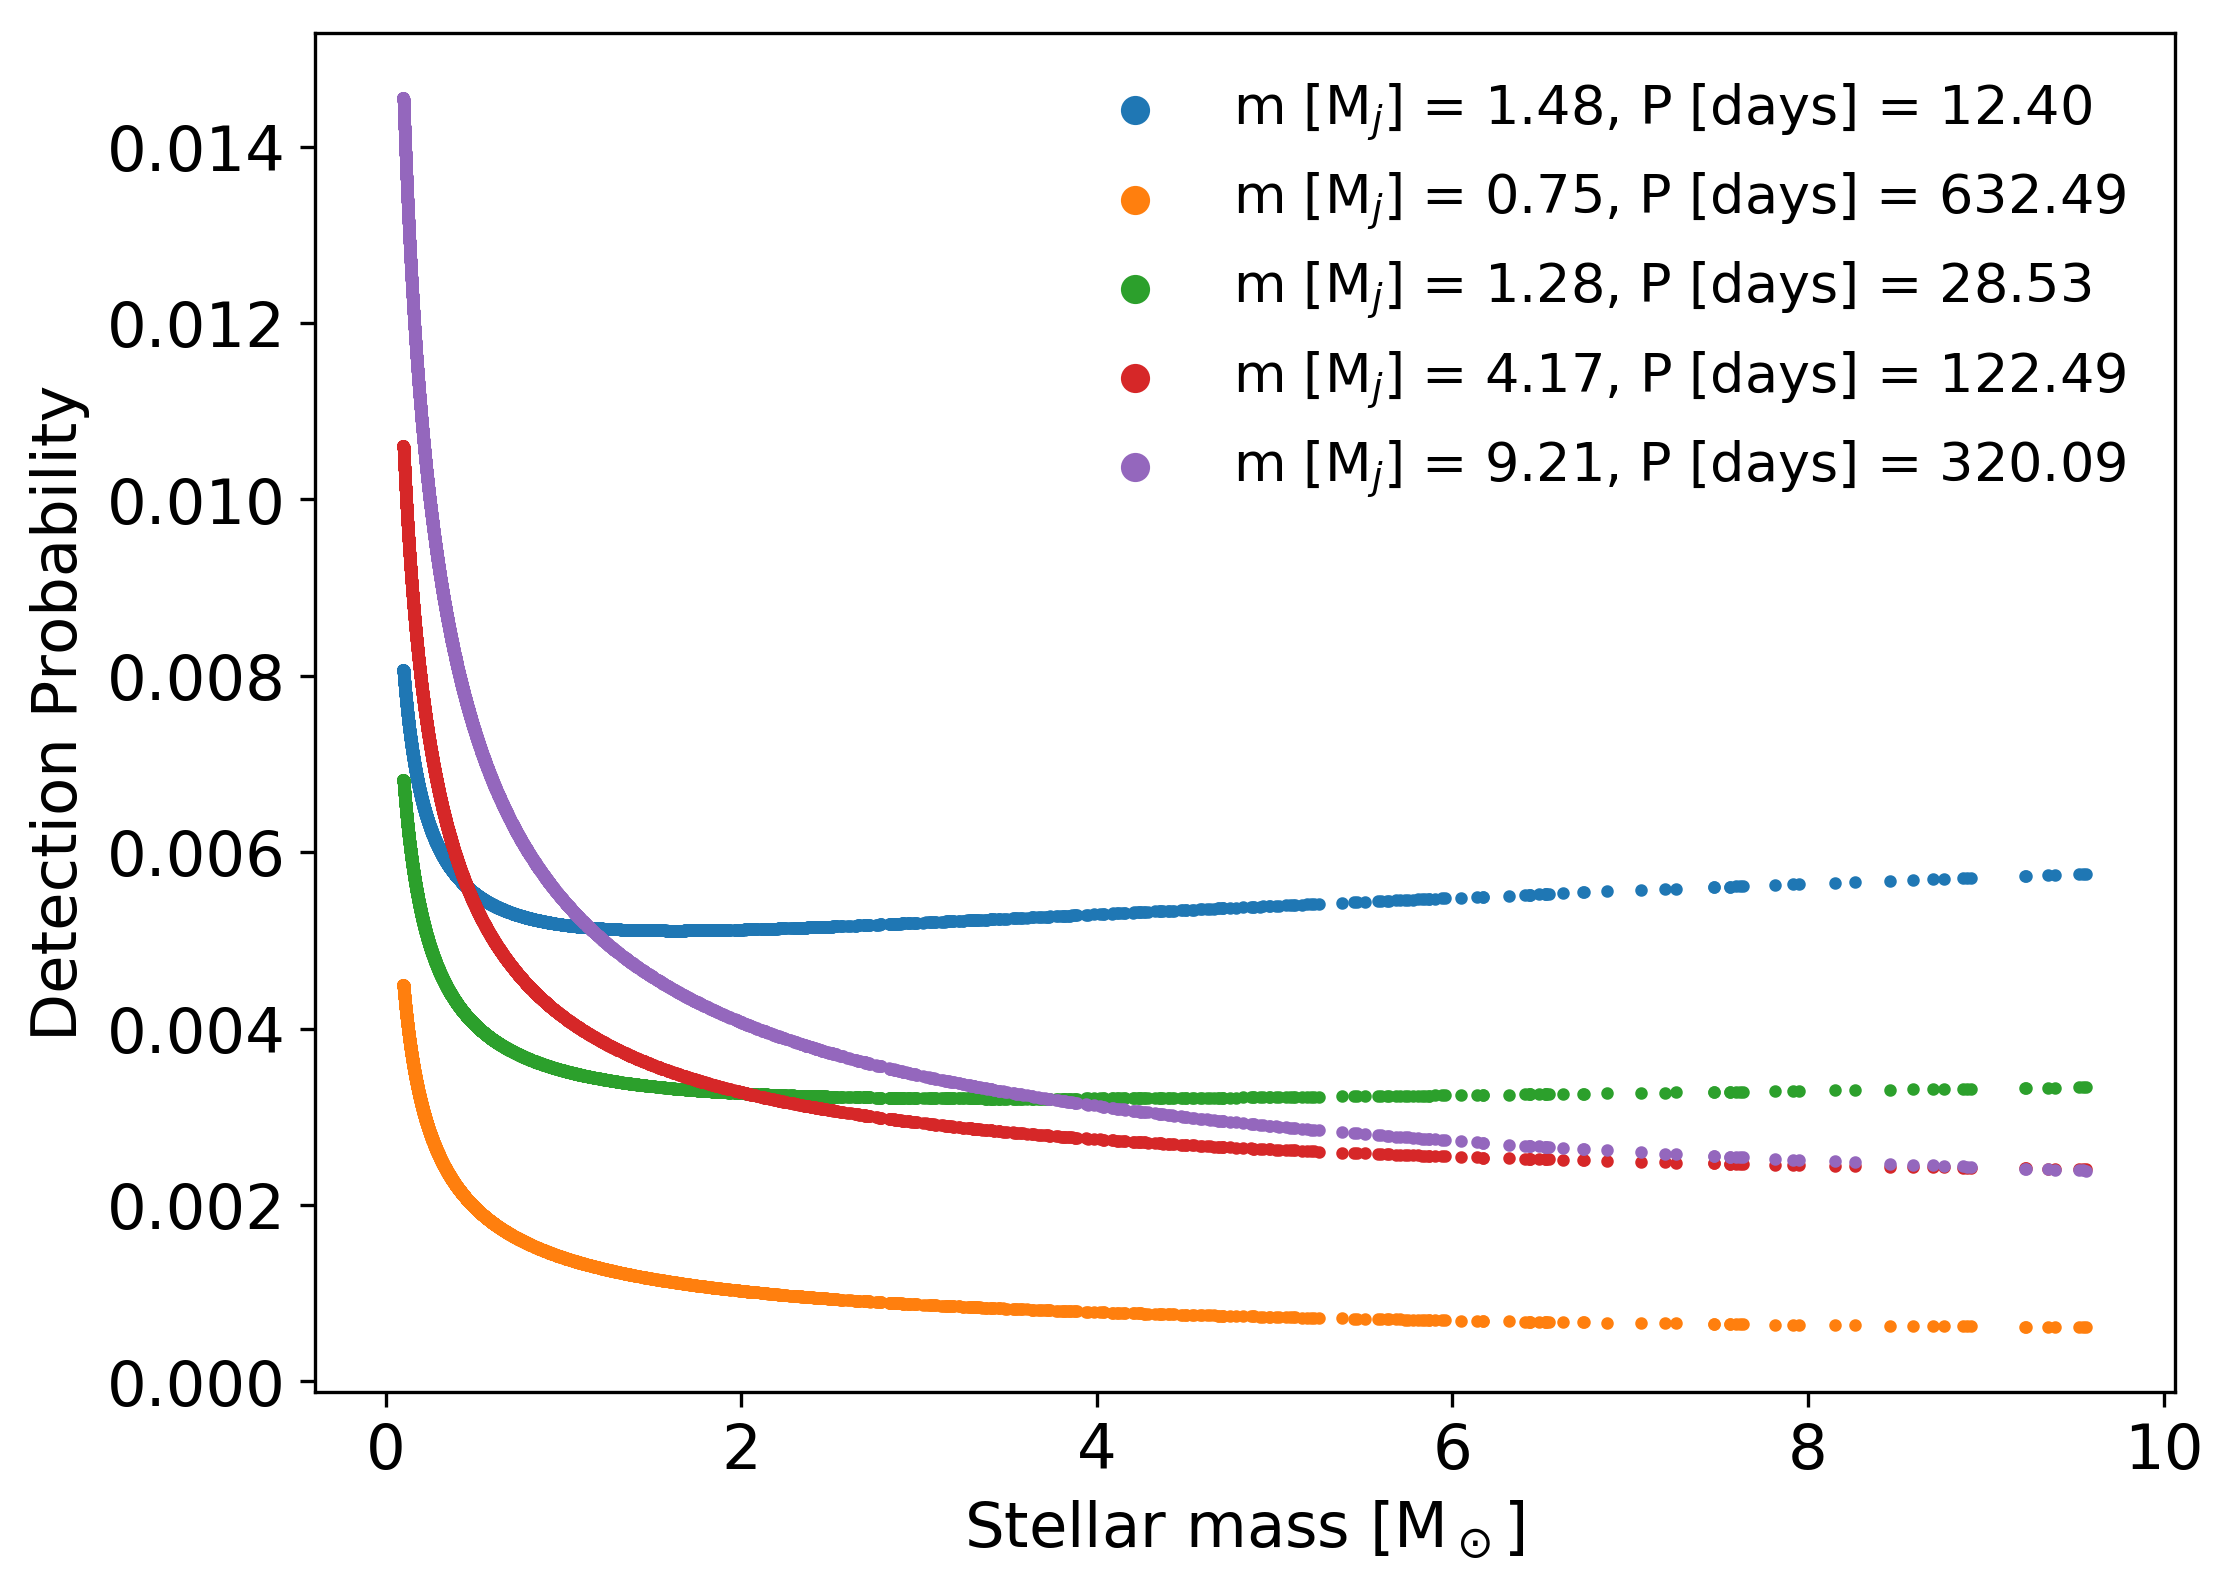
\includegraphics[width = 10cm, height = 7cm]{./Graficos/Capitulo_2/2_Exop_distributions/Monte-Carlo_KroupaNielsen.png} }}%
    \qquad
    \subfloat[]{{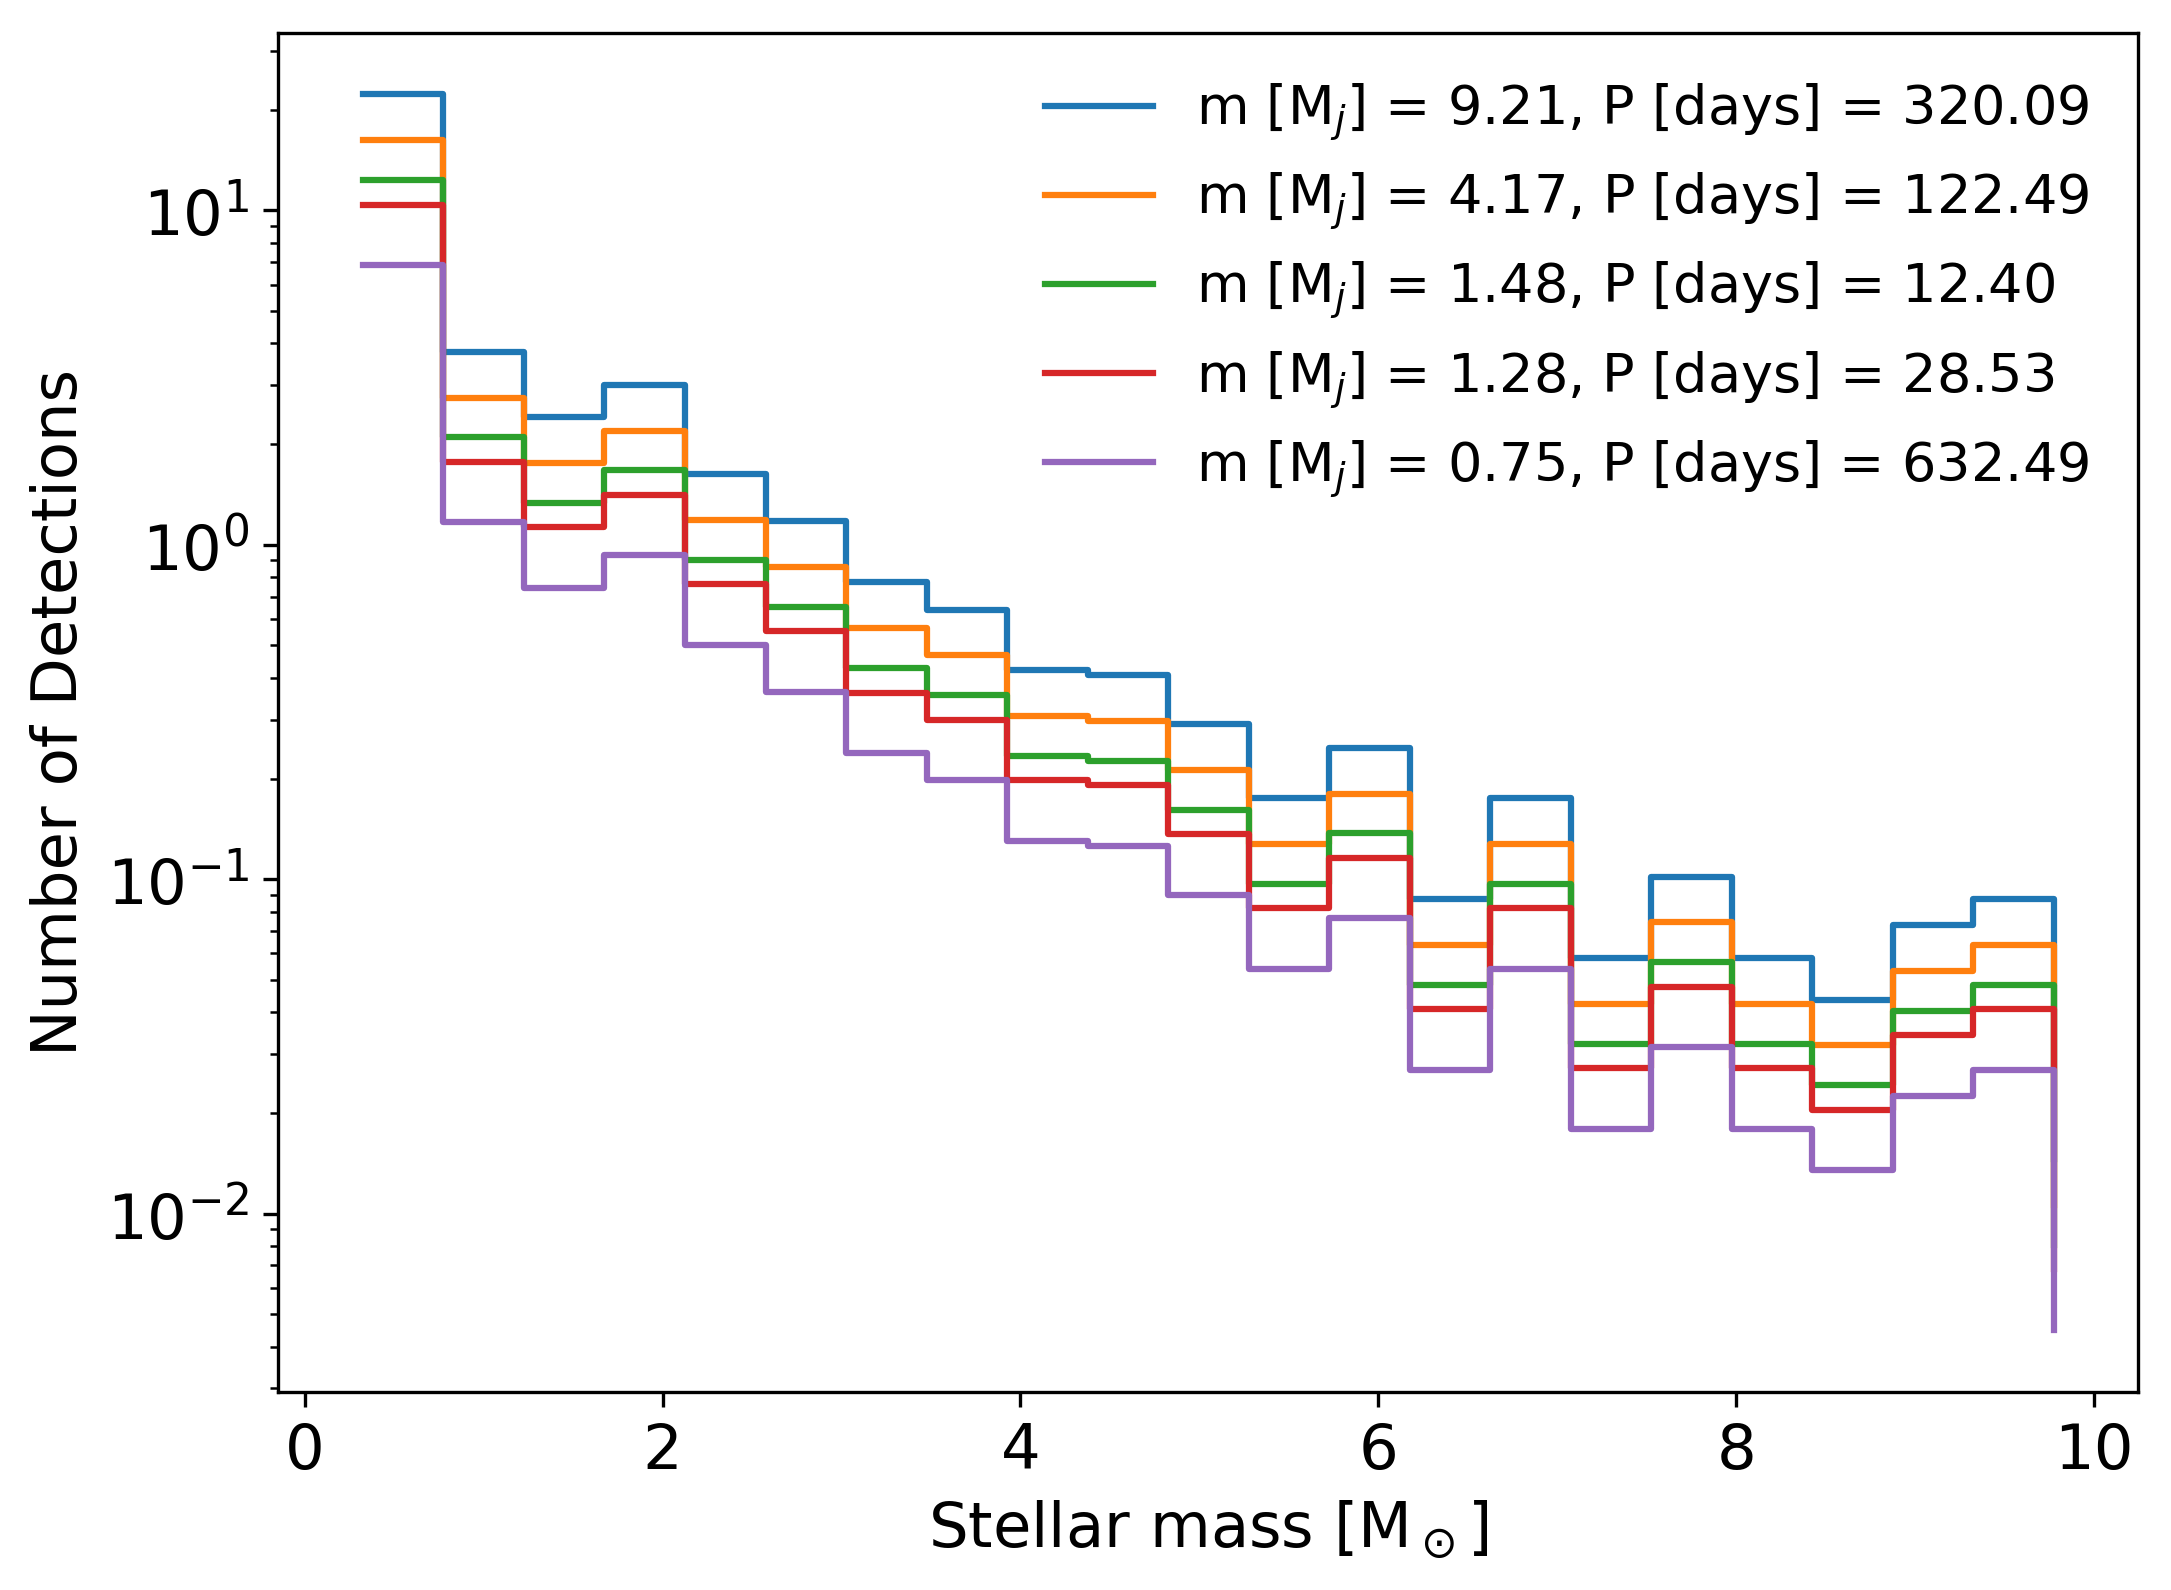
\includegraphics[width = 10cm, height = 7cm]{./Graficos/Capitulo_2/2_Exop_distributions/Monte-Carlo_KroupaNielsen_1.png} }}%
    \caption{\scriptsize{Detection probability and expected number of detections as a function of stellar mass. \textit{\textbf{(a)-panel}}: Detection probability of exoplanetary ringed systems as a function of stellar mass. Each curve corresponds to five-random-selected mass-period pairs used in \autoref{eq:FinalDetectProb}. In general, all curves follow the same trend, in which the best chance of detecting ring systems is around low-mass stars. \textit{\textbf{(b)-panel}}: Expected number of detections as a function of stellar mass. Each curve corresponds to the summed up values in each bin. The highest number of exoplanetary ringed systems are expected for stellar masses below $2 \textnormal{M}_\odot$.}}%
    \label{fig:MonteKroupaNielsen}%
\end{figure}

On the other hand, we evaluated directly \autoref{eq:FinalDetectProb} where instead of summing up each value inside a given bin, we integrate this function and use a weight to re-scale the values using the fact that as the stellar initial mass function follows a power law, it is possible to integrate each mass bin between boundaries $m_1$ and $m_2$ while leaving the total number of stars fixed i.e. $N = 10.000$, and finding the proportionality constant. This way is easier to compute the number of detections without recurring to a generation of large samples using the Monte-Carlo approach. To check this, we decided to test an exoplanet of $10\textnormal{Mj}$ and $5\textnormal{yr}$ period. First, using the Monte-Carlo process to generate the $10.000$ starts following the Kroupa distribution and evaluating \autoref{eq:FinalDetectProb} with fixed exoplanetary mass-period. After this, the detection probability was summed up in bins of $0.5M_\odot$ and the result is shown in \autoref{fig:MonteAnalytic_1}. However, for the second case, \autoref{eq:FinalDetectProb} was directly evaluated in a regular stellar mass array without any Monte-Carlo approach, and the detection probability was integrated fixing the total number of stars to re-scale each bin. The final result is shown in \autoref{fig:MonteAnalytic_1}. Both approaches lead to similar results, although in the case of the analytic form the slope is a bit steeper due to the fact that we are considering a fixed number of stars per bin derived from the continuity equation of the power law as explained before. If we reproduce the Monte-Carlo process several times we will eventually end up in this case. In brief, the analytic form approach will be used to study the dependence of this detection probability and the number of expected detections as a function of the fifth probability which was not introduced here and it is related to the lifetime of the planetary rings.\\

\begin{figure}[!ht]%
    \centering
    \subfloat{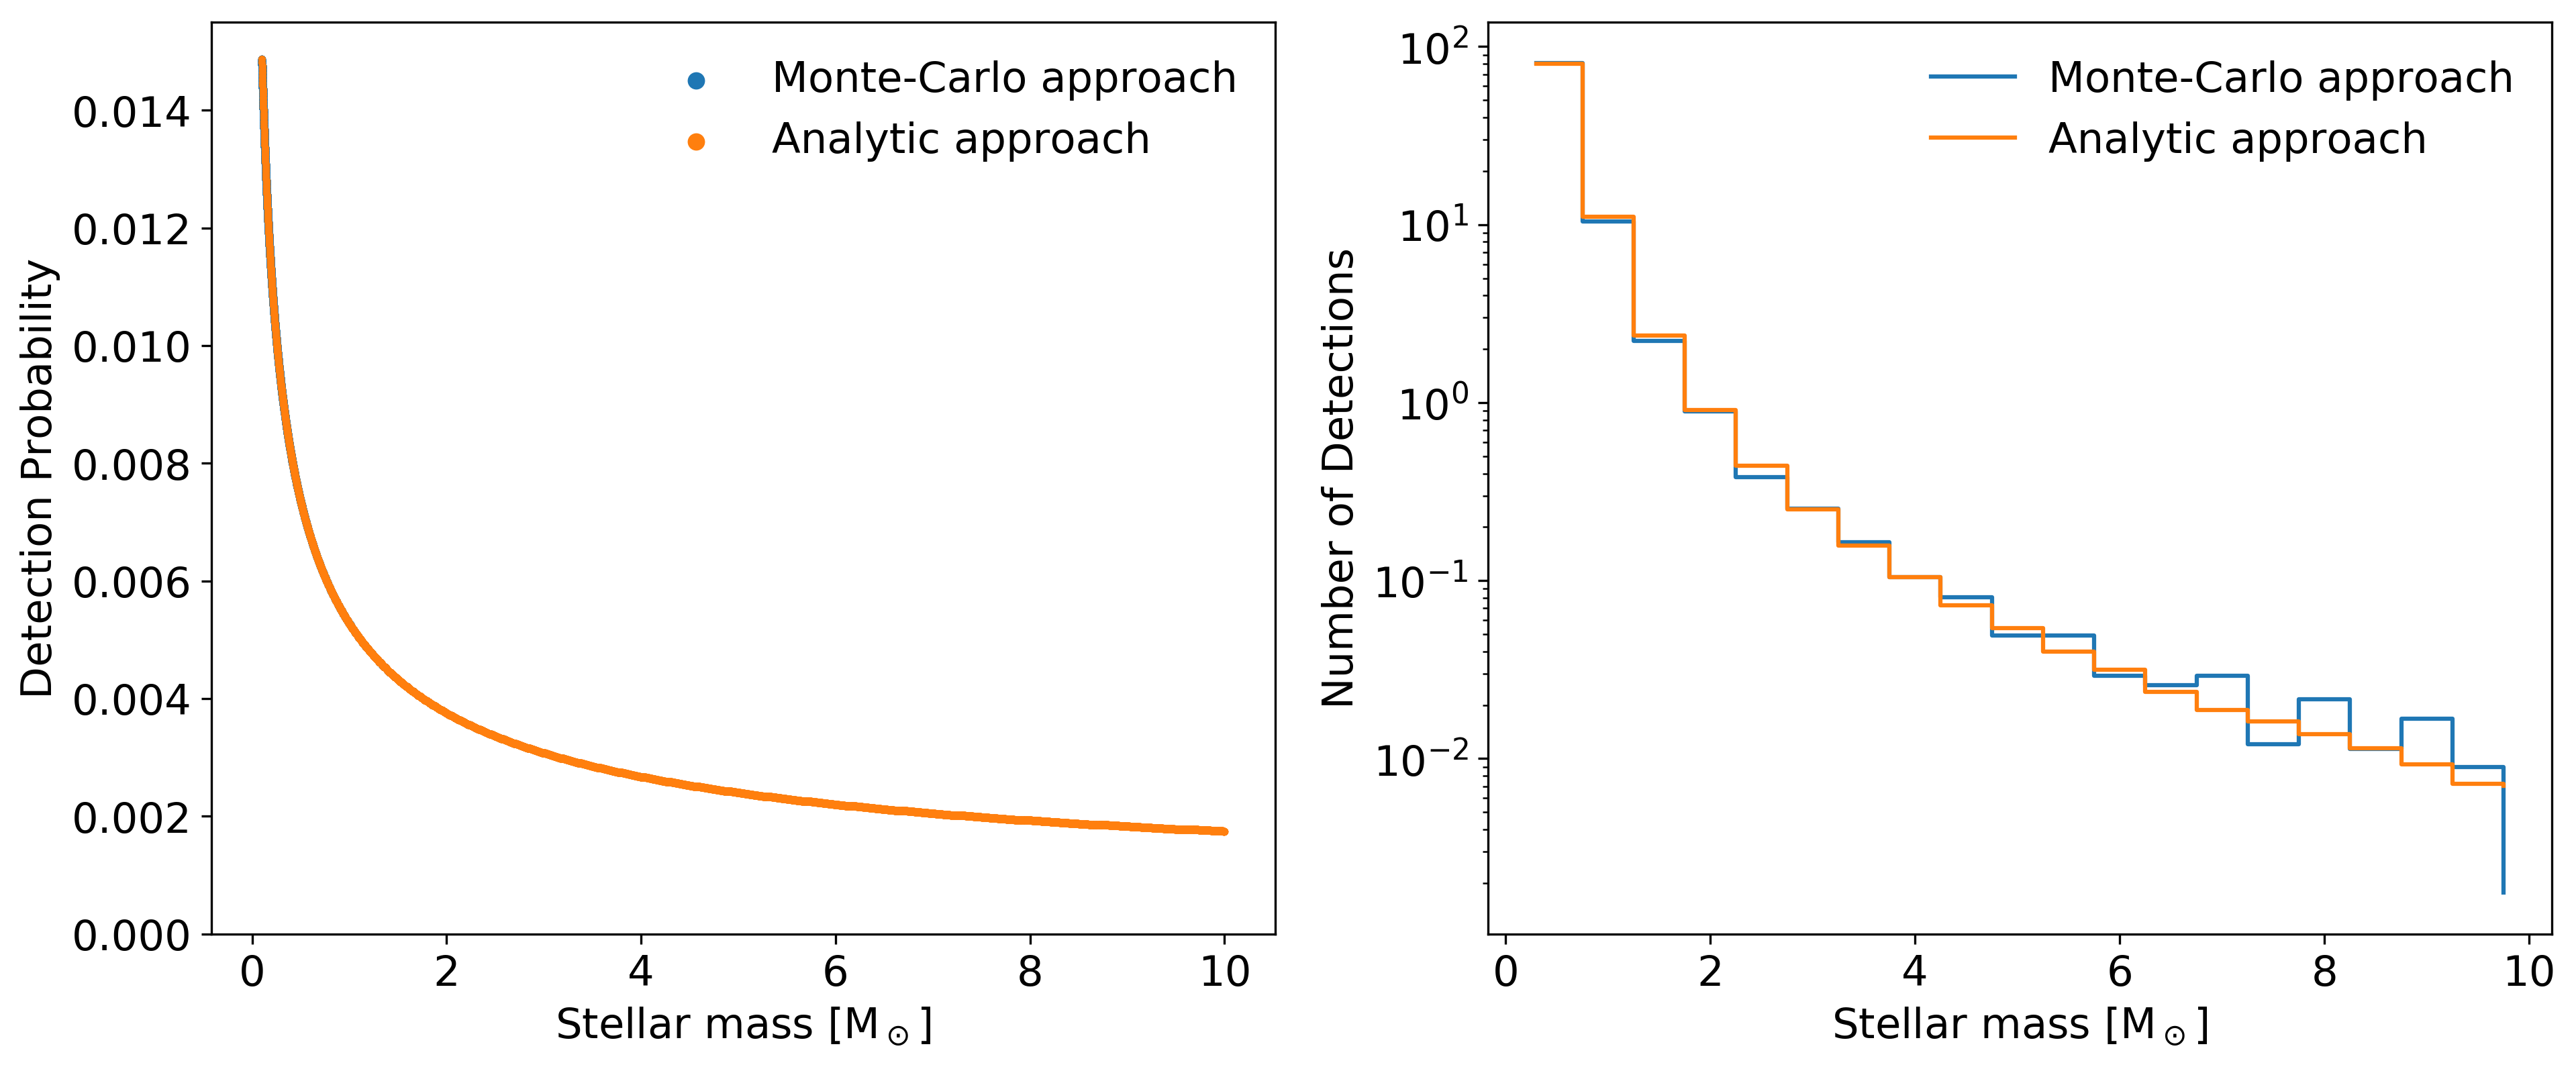
\includegraphics[width = 16cm, height = 6.5cm]{./Graficos/Capitulo_2/2_Exop_distributions/MC_Analytic.png} }%
    \caption{\scriptsize{Detection probability and expected number of detections as a function of stellar mass for an exoplanet of $10 \textnormal{Mj}$ mass and $5 \textnormal{yr}$ period. \textit{\textbf{left}}: Detection probability of an exoplanetary ringed system as a function of stellar mass. The blue and orange curves corresponds to one mass-period pair used in \autoref{eq:FinalDetectProb}. \textit{\textbf{right}}: Expected number of detections as a function of stellar mass. This is generated using the Monte-Carlo and analytic approaches.}}%
    \label{fig:MonteAnalytic_1}%
\end{figure}

% \begin{figure}[!ht]%
%     \centering
%     \subfloat[]{{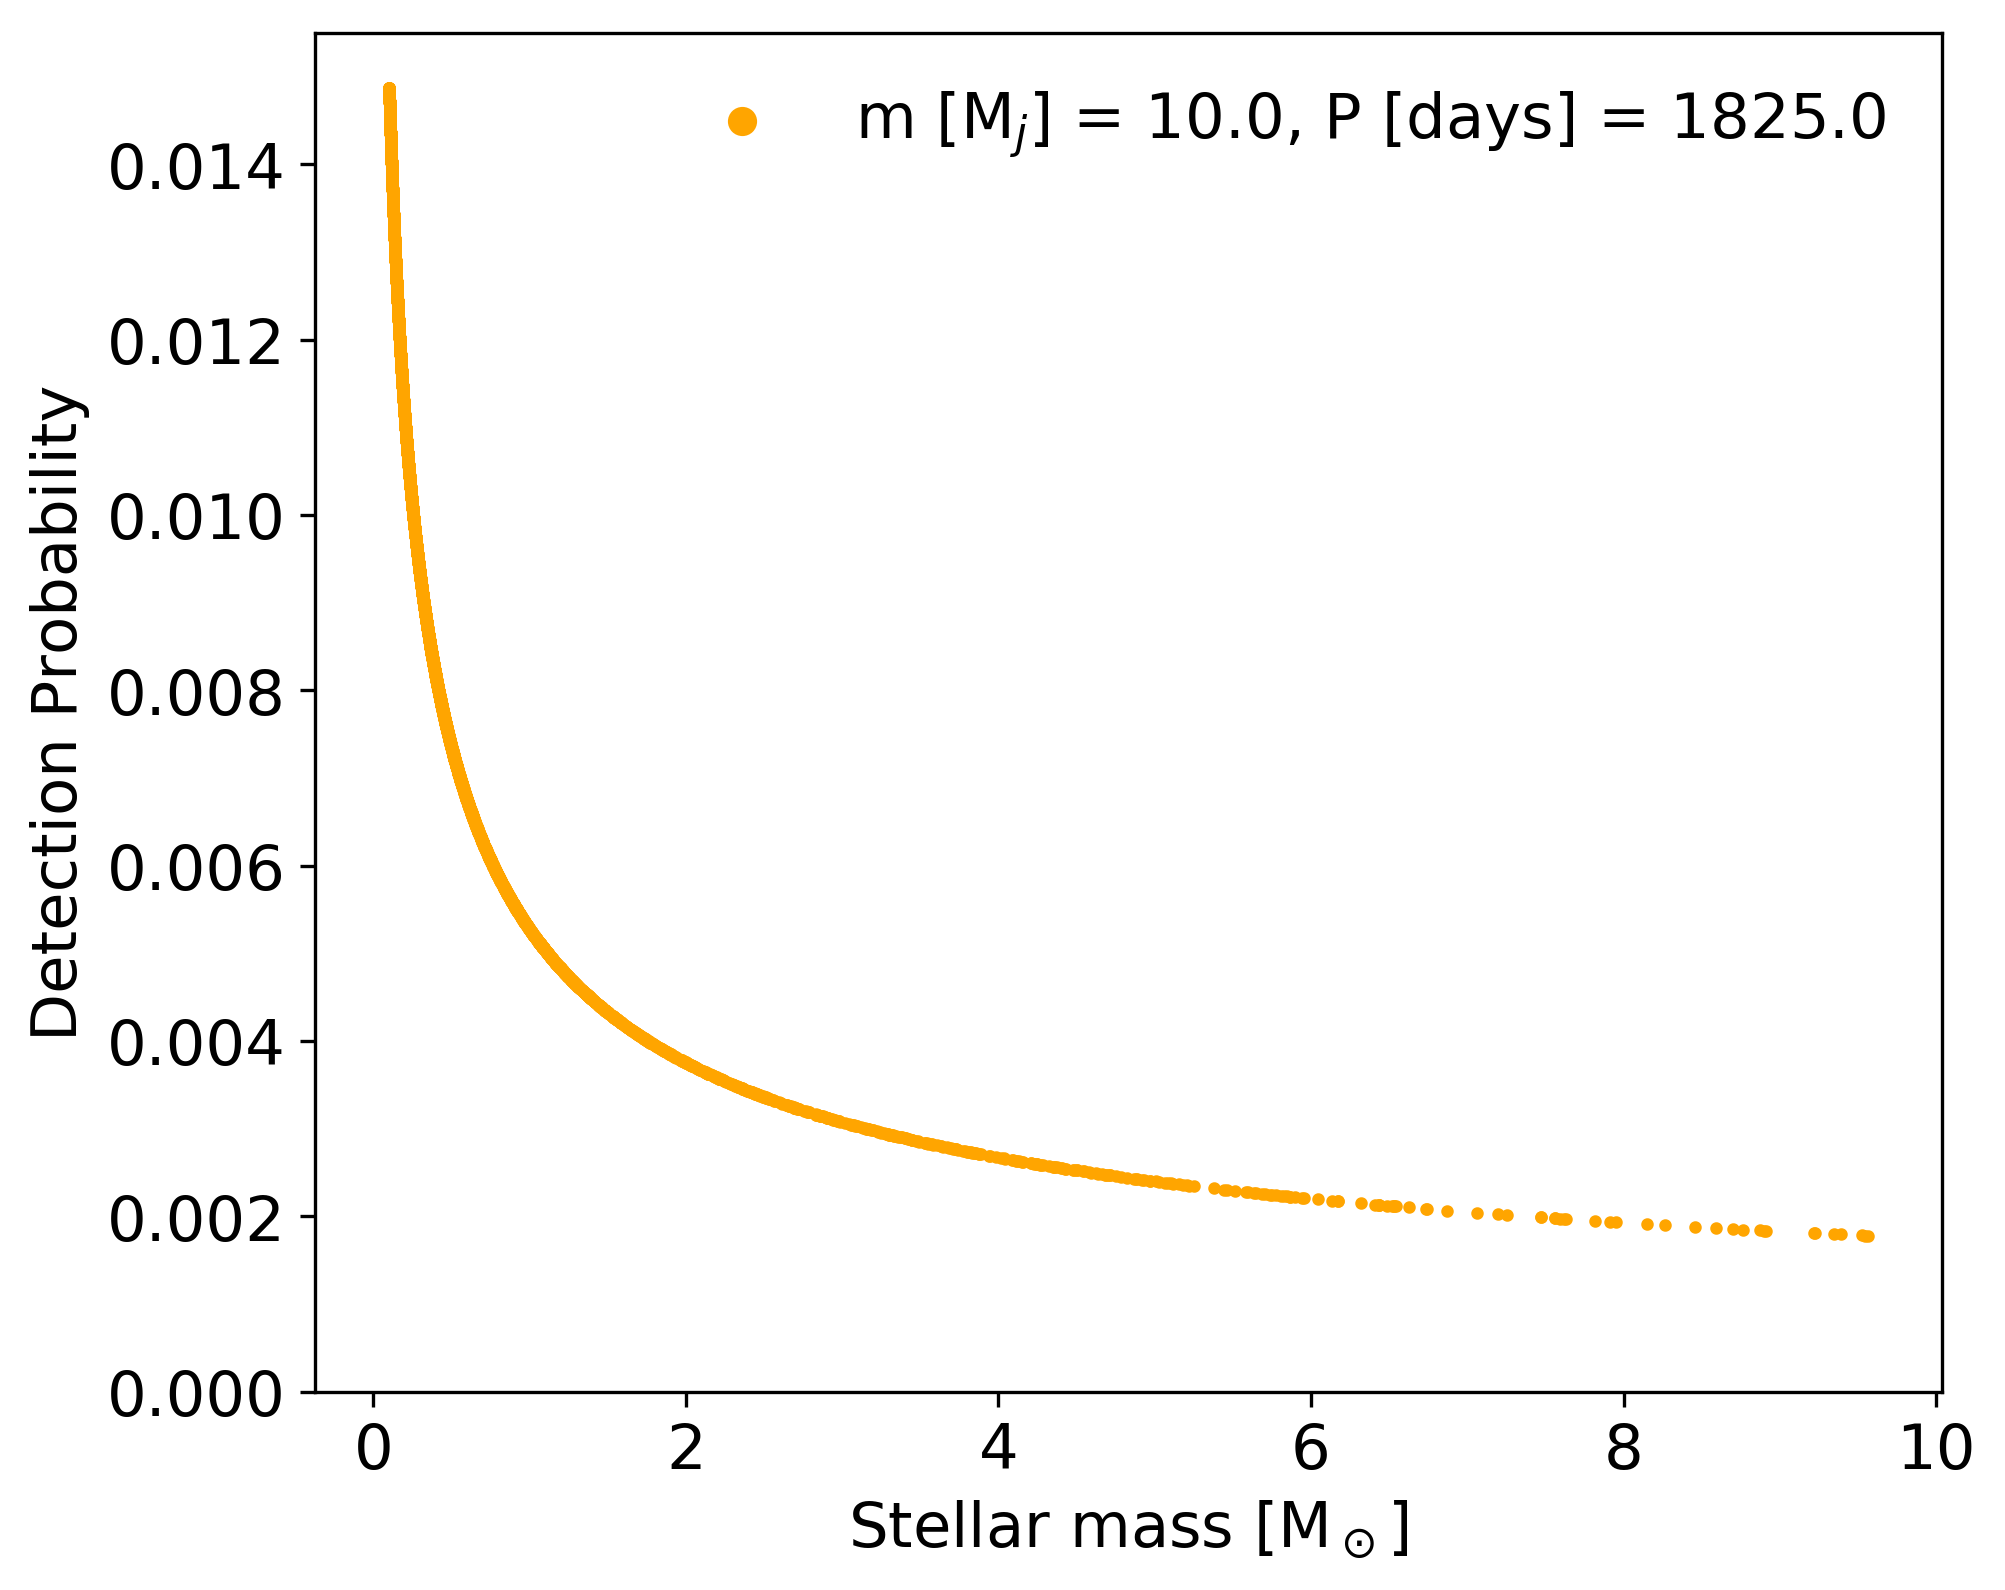
\includegraphics[width = 10cm, height = 7cm]{./Graficos/Capitulo_2/2_Exop_distributions/Monte-Carlo_KroupaNielsen_2.png} }}%
%     \qquad
%     \subfloat[]{{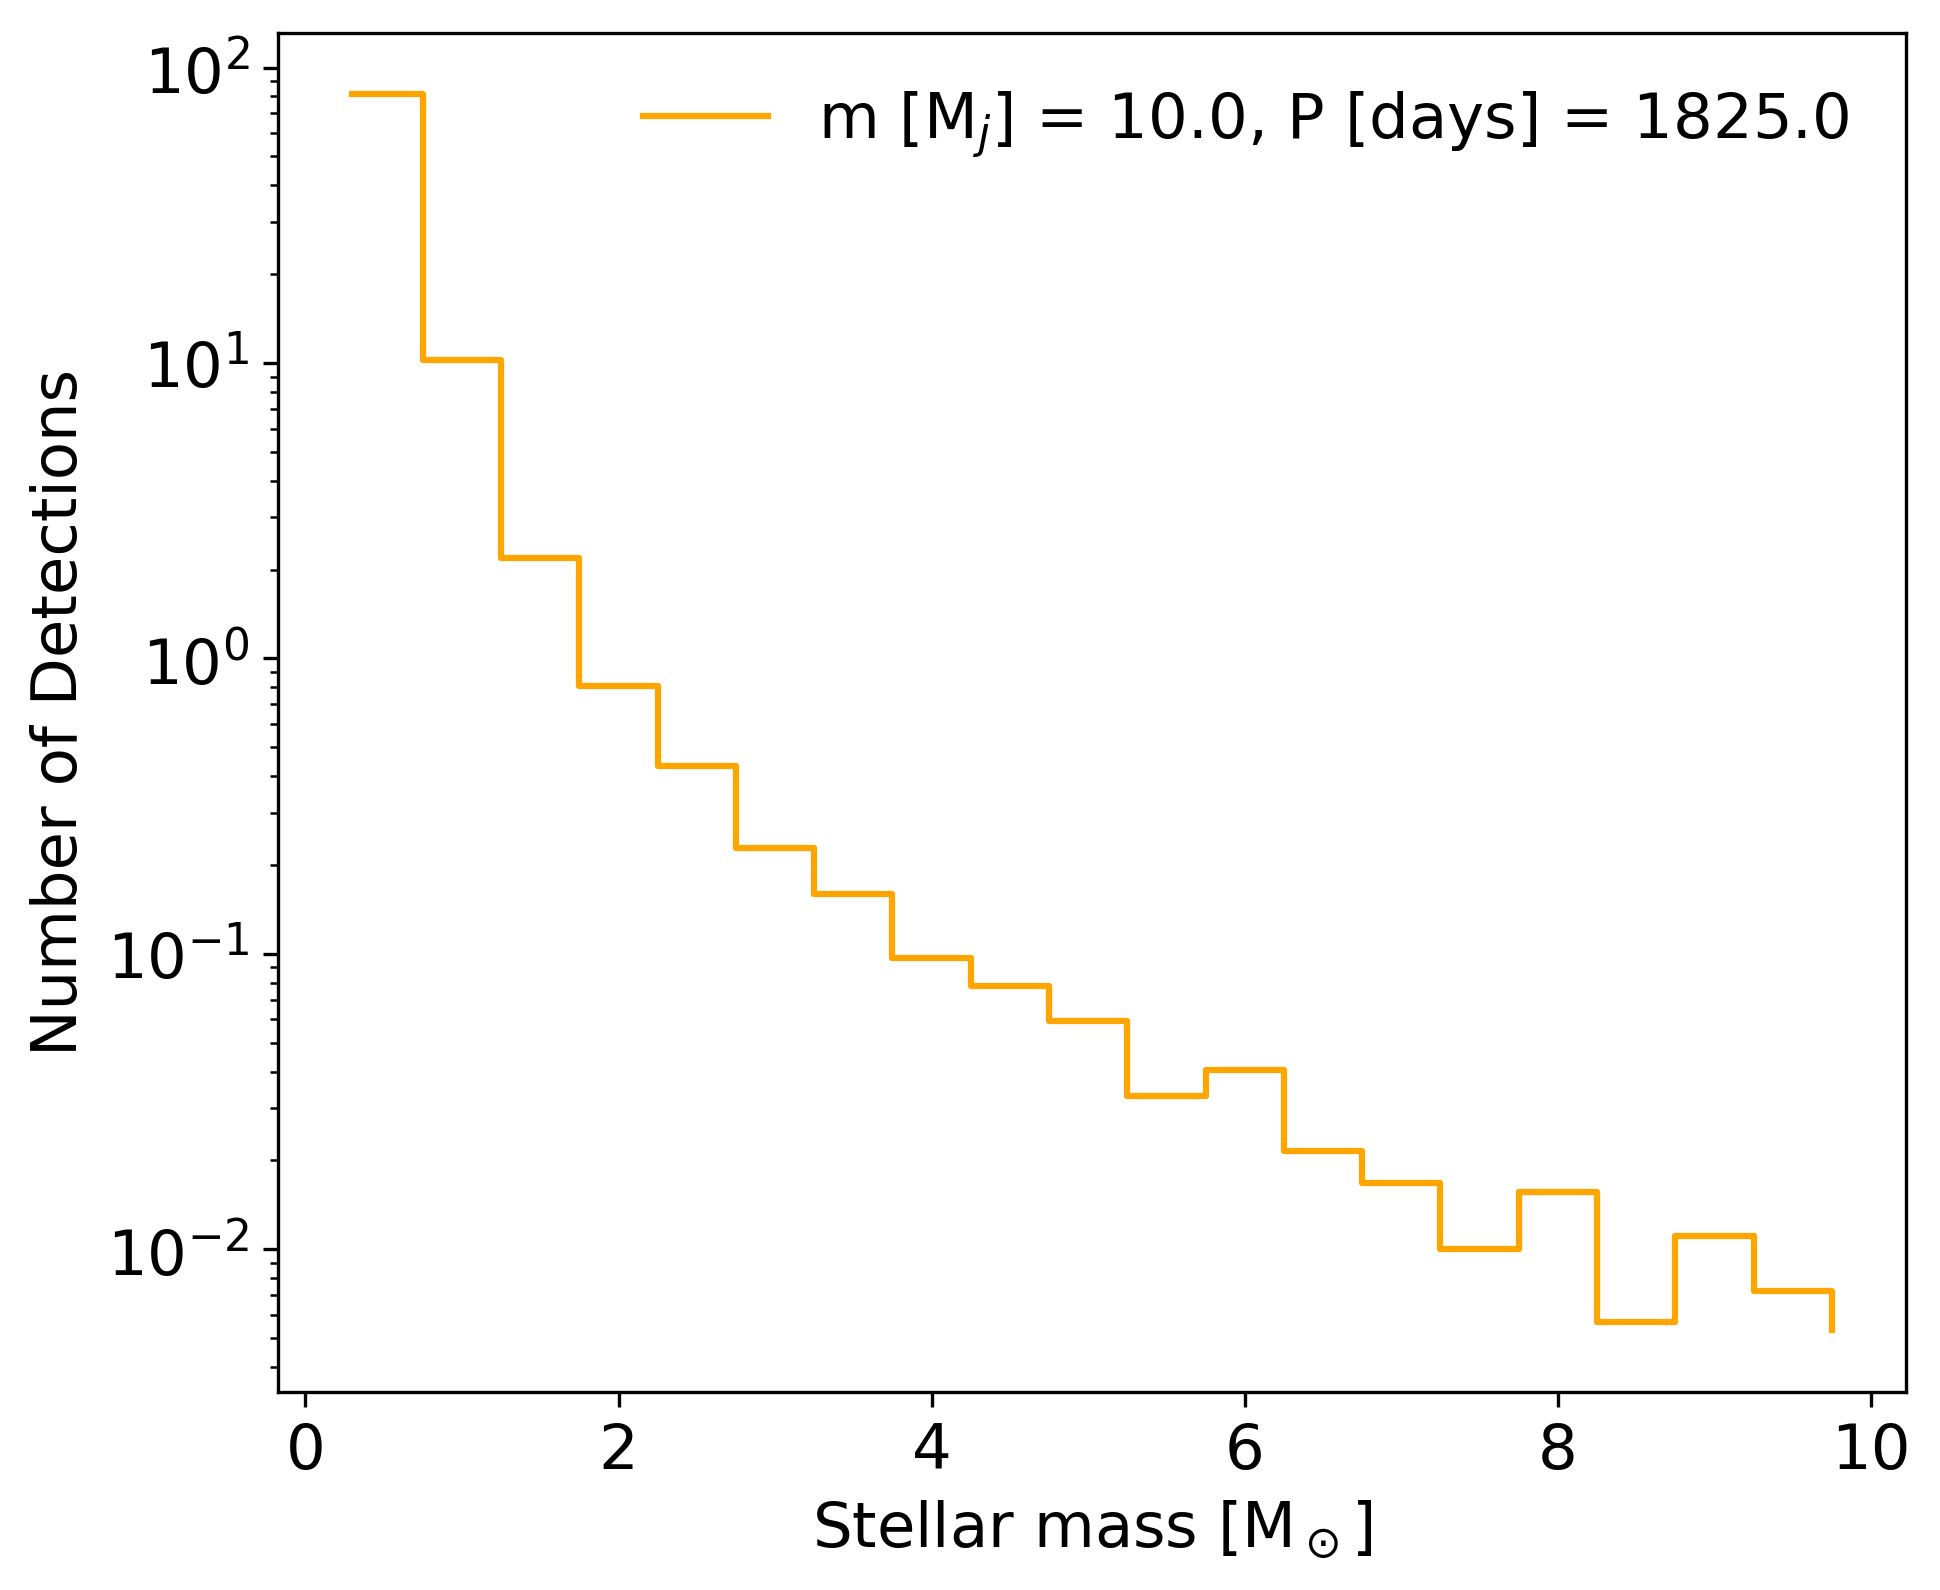
\includegraphics[width = 10cm, height = 7cm]{./Graficos/Capitulo_2/2_Exop_distributions/Monte-Carlo_KroupaNielsen_3.png} }}%
%     \caption{\scriptsize{Detection probability and expected number of detections as a function of stellar mass for an exoplanet of $10 \textnormal{Mj}$ mass and $5 \textnormal{yr}$ period. \textit{(a)-panel}: Detection probability of an exoplanetary ringed system as a function of stellar mass. The curve corresponds to one mass-period pair used in \autoref{eq:FinalDetectProb}. \textit{(b)-panel}: Expected number of detections as a function of stellar mass. This is generated using the Monte-Carlo approach and is shown to compare the analytic results obtained in \autoref{fig:MonteAnalytic_1}.}}%
%     \label{fig:MonteAnalytic_1}%
% \end{figure}
% 
% \begin{figure}[!ht]%
%     \centering
%     \subfloat[]{{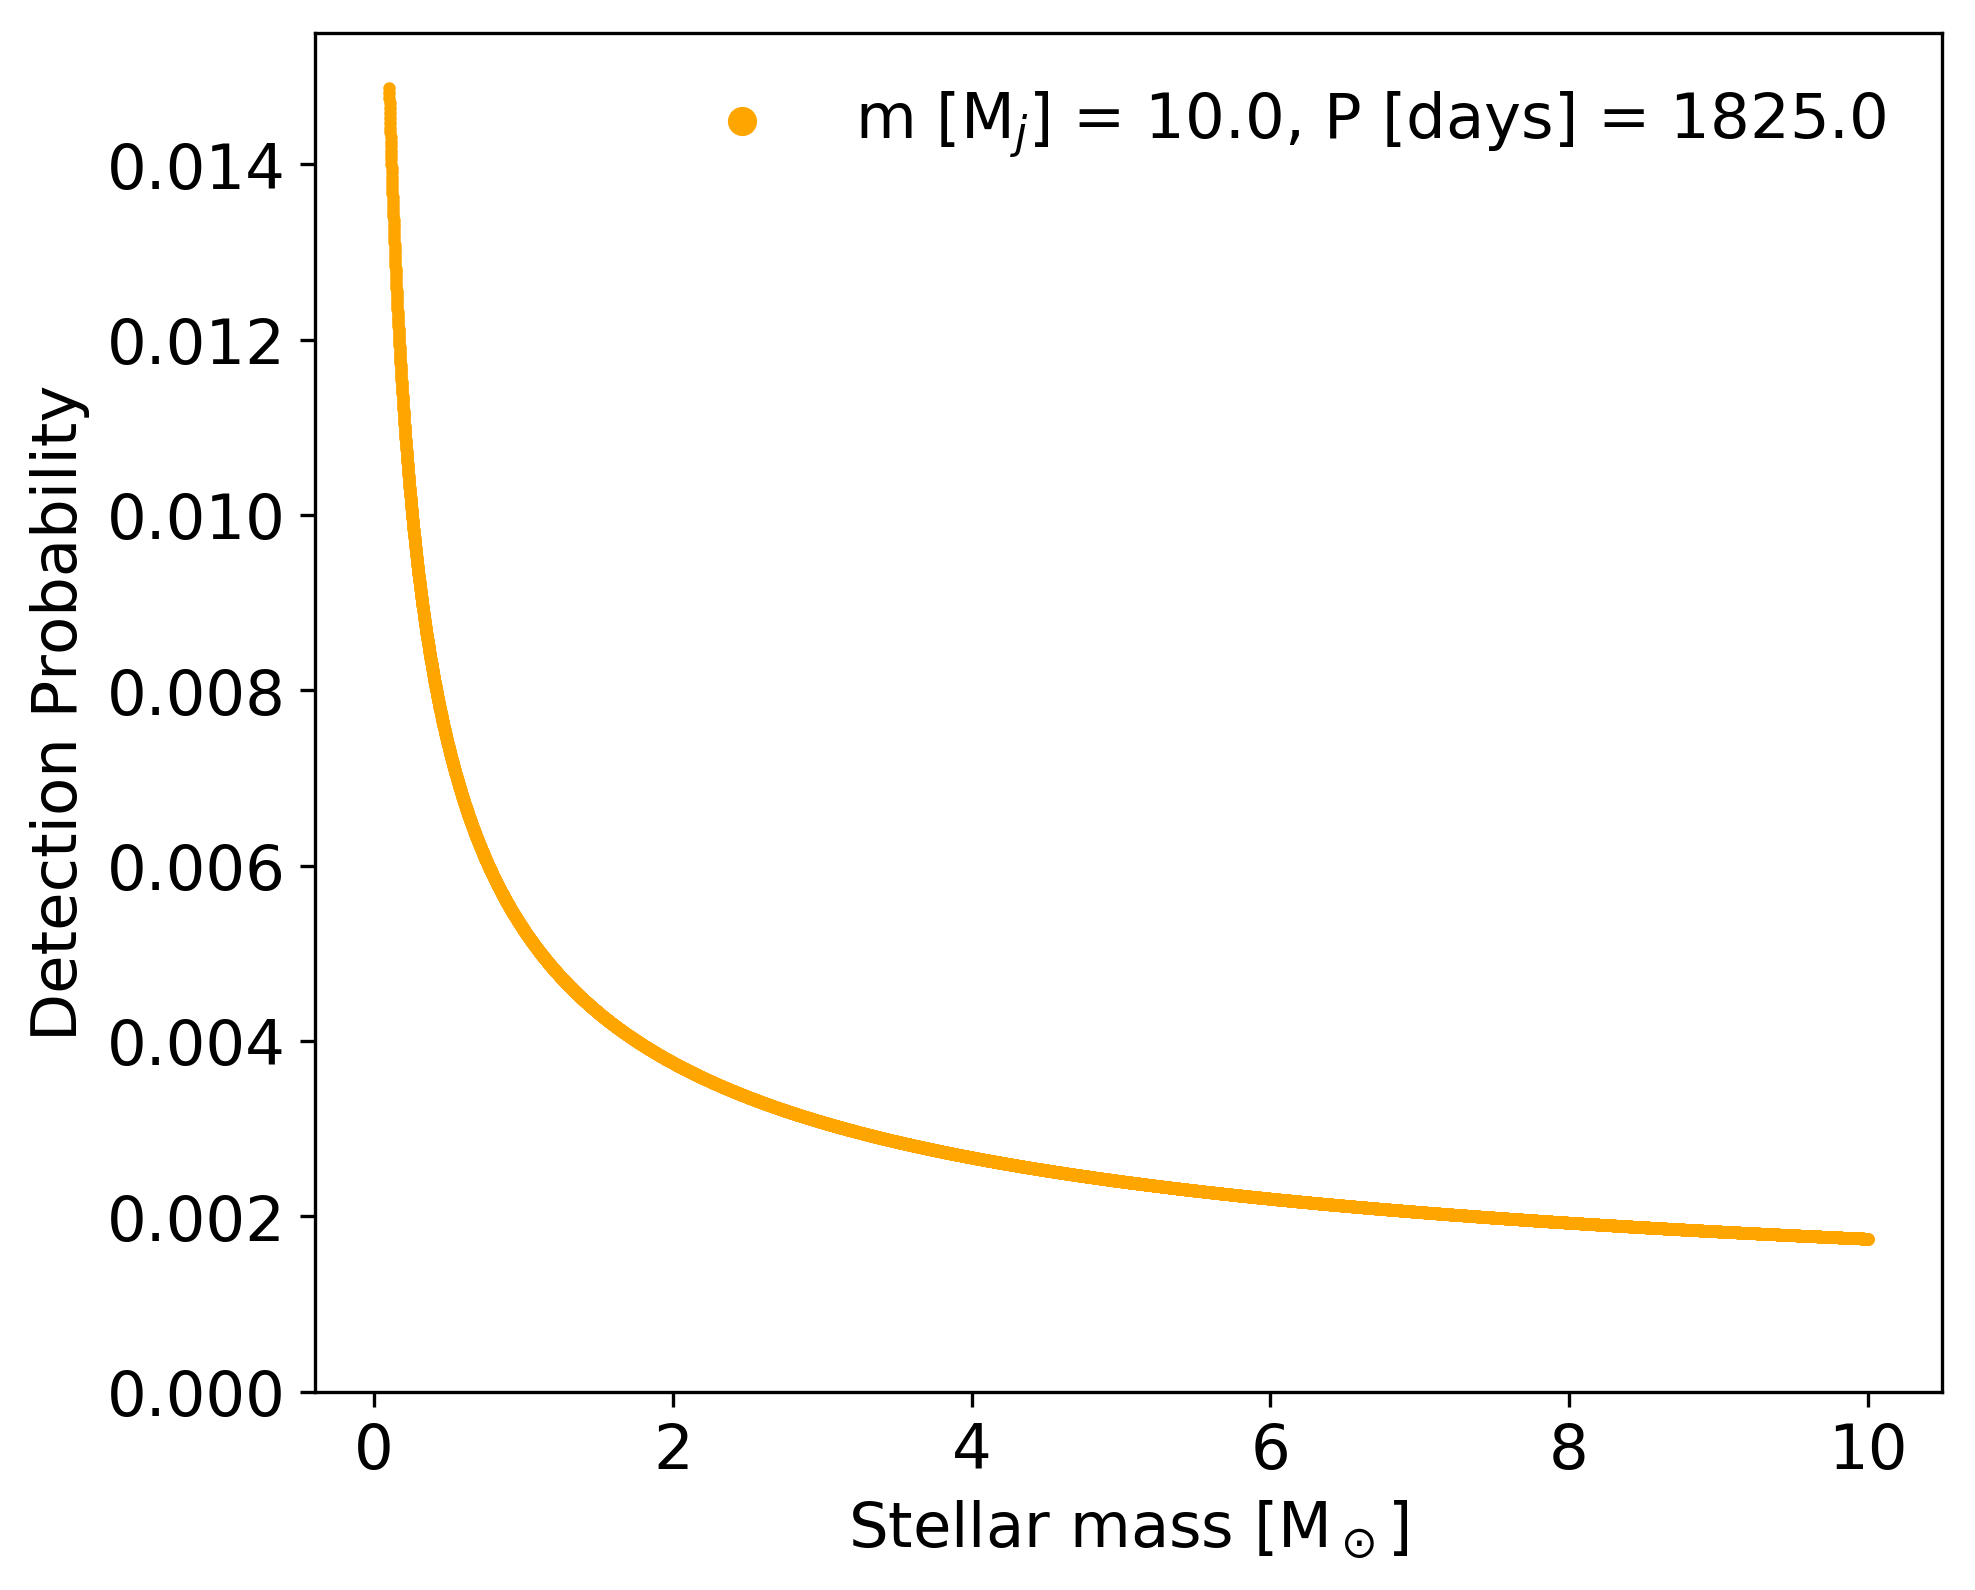
\includegraphics[width = 10cm, height = 7cm]{./Graficos/Capitulo_2/2_Exop_distributions/Analytic_Kroupa_Nielsen.png} }}%
%     \qquad
%     \subfloat[]{{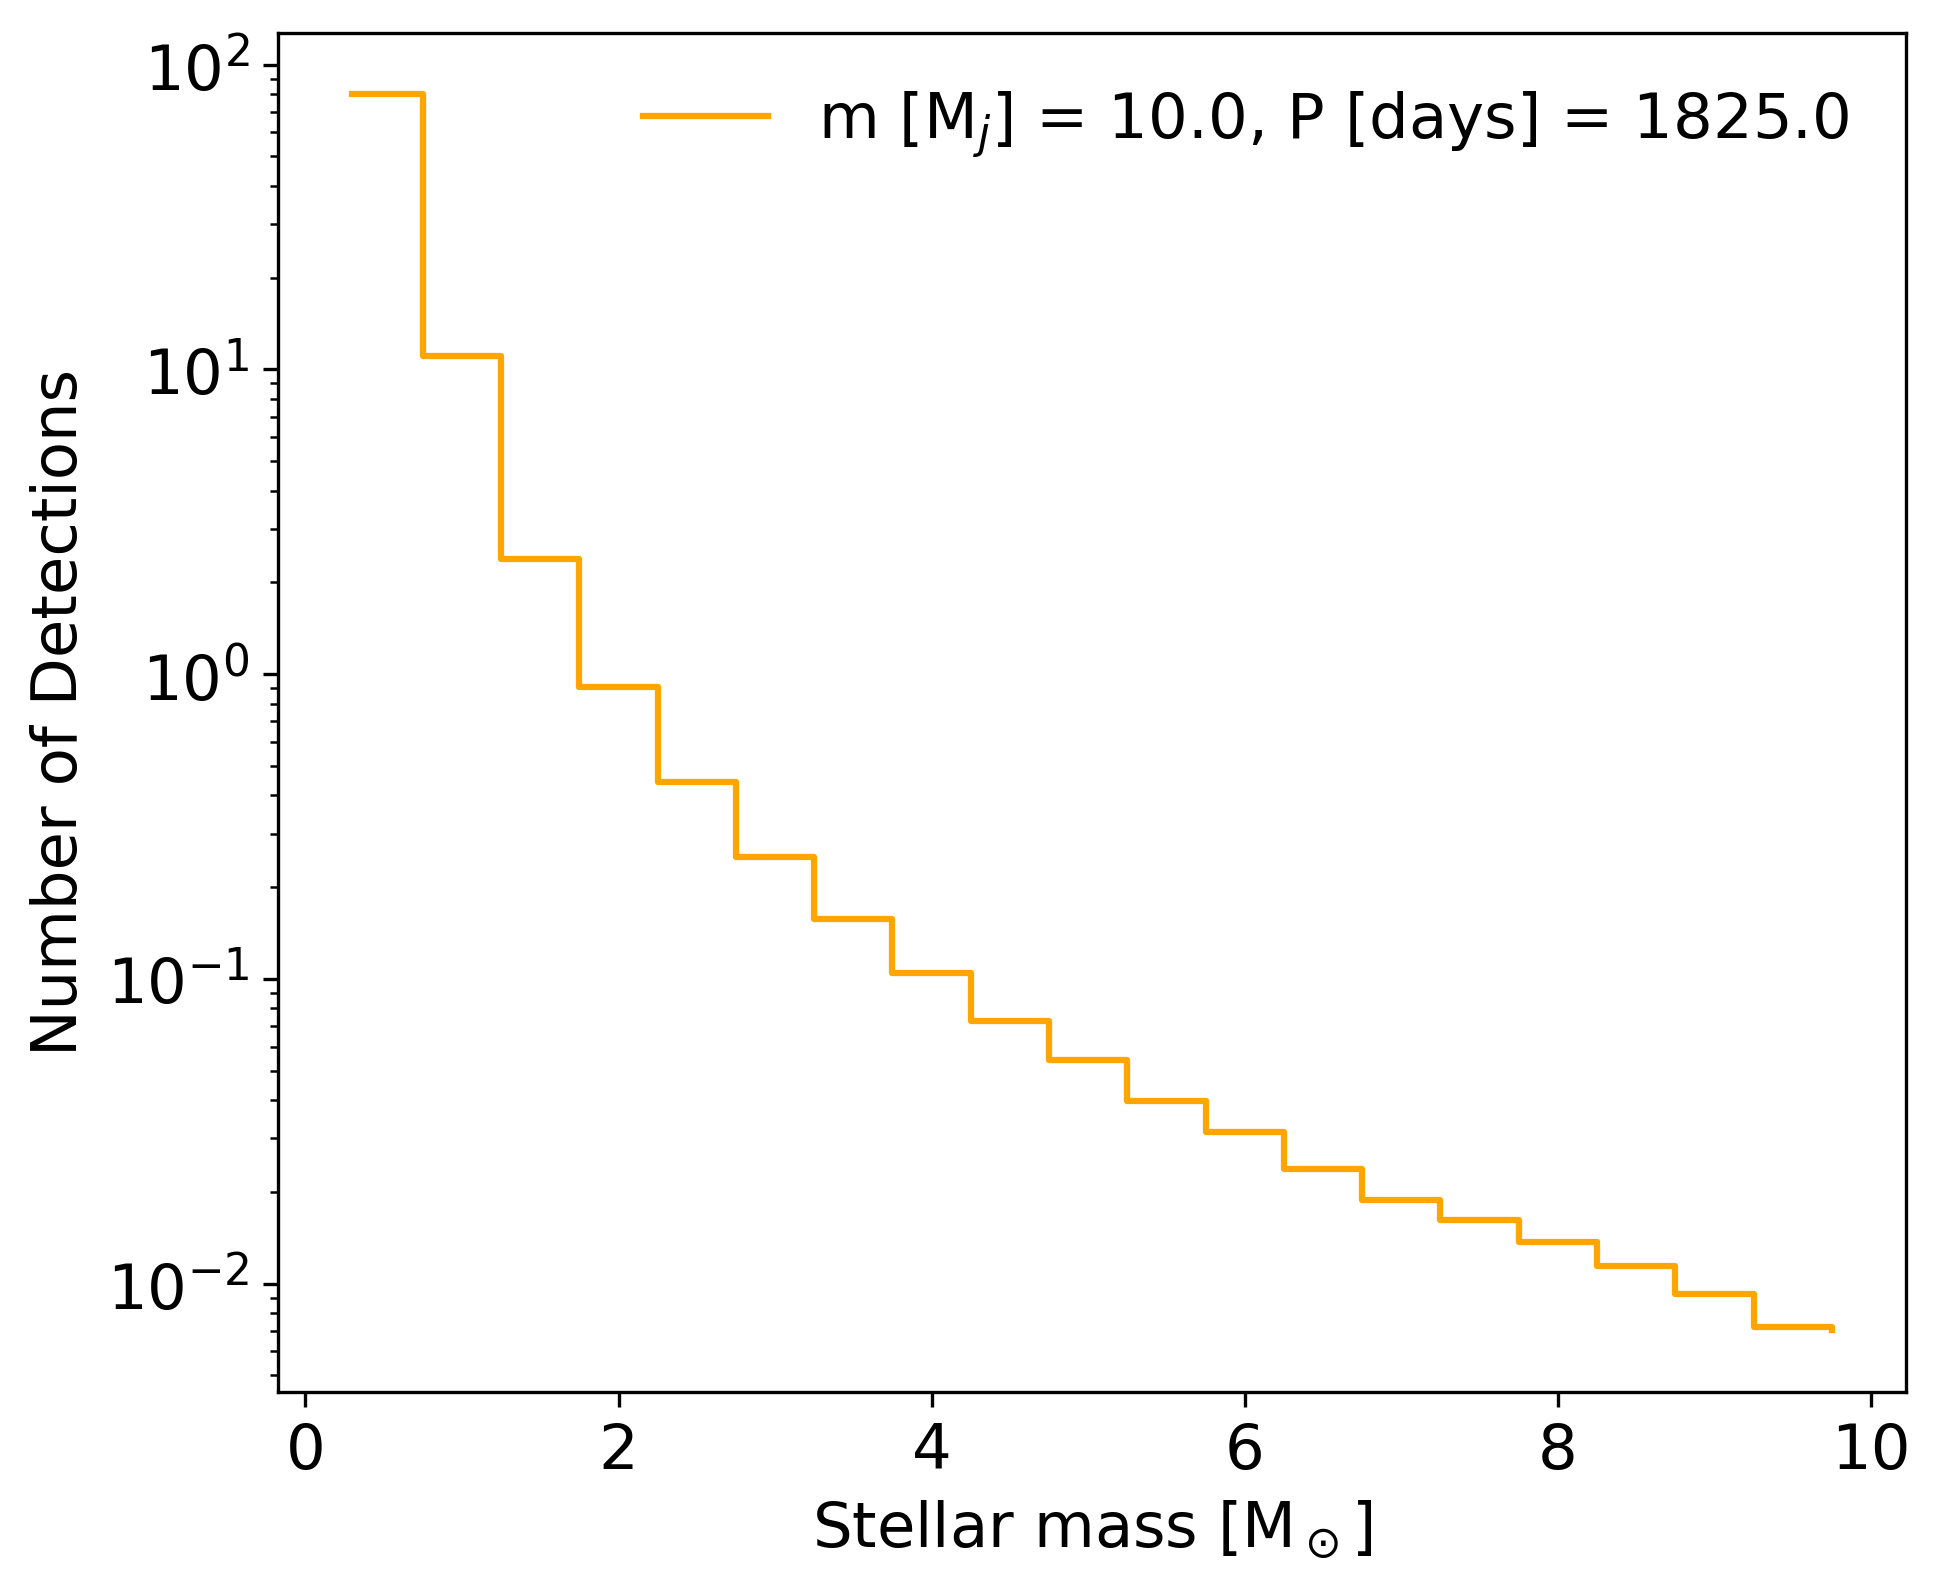
\includegraphics[width = 10cm, height = 7cm]{./Graficos/Capitulo_2/2_Exop_distributions/Analytic_Kroupa_Nielsen_1.png} }}%
%     \caption{\scriptsize{Detection probability and expected number of detections as a function of stellar mass for an exoplanet of $10 \textnormal{Mj}$ mass and $5 \textnormal{yr}$ period using an analytic approach. \textit{(a)-panel}: Detection probability of an exoplanetary ringed system as a function of stellar mass. The curve corresponds to one mass-period pair used in \autoref{eq:FinalDetectProb}. \textit{(b)-panel}: Expected number of detections as a function of stellar mass. This is generated using an analytic approach instead of the Monte-Carlo simulation shown in \autoref{fig:MonteAnalytic_1}.}}%
%     \label{fig:MonteAnalytic_1}%
% \end{figure}

Besides, tt was pointed out in \autoref{subsec:RingsSec} that there is no general consensus on the timescale in which planetary rings are formed or for how long they survive. However, based on evidence from our own solar system there is a range of possible values which will give a glimpse on this value. We decided to test how the detection probability and the number of detections change for different values. In \autoref{fig:Rings_Prob} each line was computed using the last method, avoiding the Monte-Carlo calculation for different rings' lifetime spanning from $1\times 10^5$yr to $1\times 10^7$yr because it was the most reliable range of values found in the literature. The case in which the fifth probability is not taken into account corresponds to an infinite timescale. It is clear that the younger the exoplanetary rings, the lower the probability of detecting them around the stellar system because as was shown in \autoref{eq:Prob_5} this probability is computed as a ratio between the rings' lifetime and the stellar age. Thus, the larger the timescale, the larger the probability, and so the detections. This is really important because depending on this value we can expect a different number of transits in a certain stellar mass range. However, it is worth noting that the highest probability is achieved towards the small stellar mass values.\\

\begin{figure}[!ht]
\centering
  \subfloat{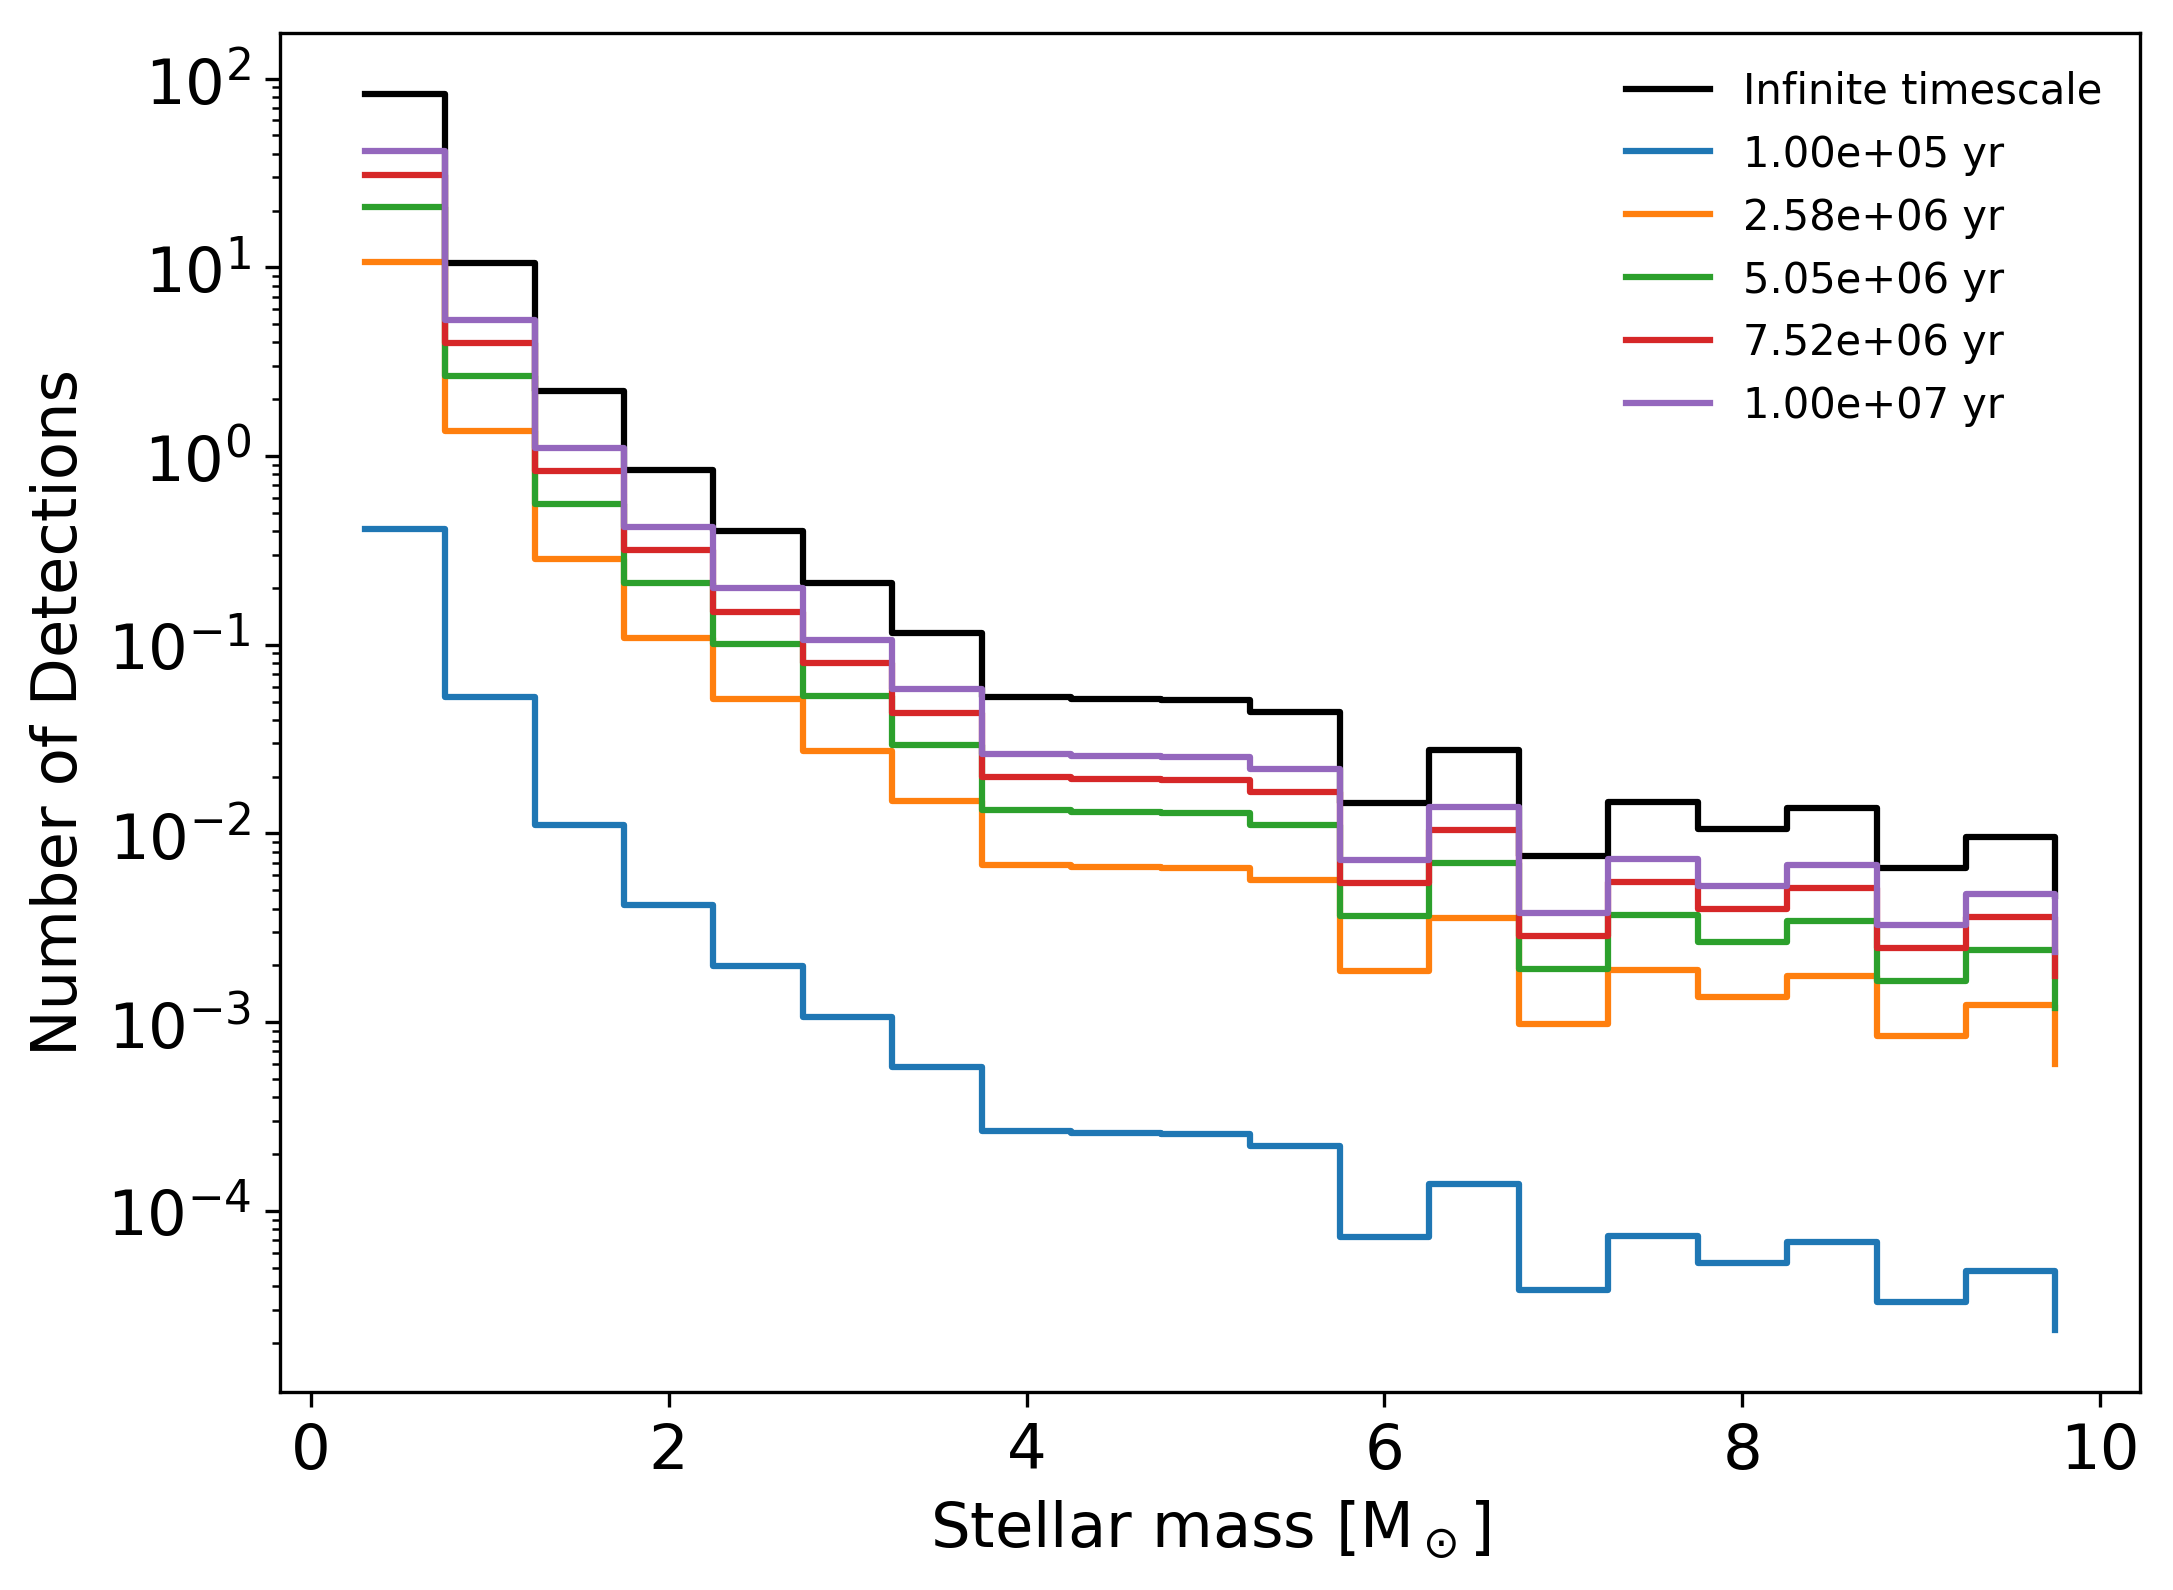
\includegraphics[width = 12cm, height = 9cm]{./Graficos/Capitulo_2/2_Exop_distributions/Analytic_rings_Kroupa_Nielsen.png}} 
\caption{\scriptsize{Expected number of detections as a function of stellar mass accounting for the rings' lifetime contribution. $0.0 \textnormal{yr}$ corresponds to a system where the rings are in place since the stellar and planet formation process until it is observed. Different times represent the lifespan of the exoplanetary rings. As the lifetime increases, also does the number of detections as the chance to observe an exoring in the system increases, converging to its maximum value if we assume the exorings to have an infinite lifetime.}}
\label{fig:Rings_Prob}
\end{figure}

In conclusion, we present different ways to calculate the expected number of detections. However, we decided to stick to the analytic form instead of using the Monte-Carlo process just for simplicity though both methods lead to the same results in overall. Also, there are different ways to generate the stellar masses using the Salpeter or Kroupa's initial mass functions. All the methods explained above are available in the Git-Hub repository \url{https://github.com/Jurgenvilla/Exoplanet-Rings-and-Gaia}. It is, however, worth noting that the main conclusion from this analysis relies on the fact that the number of planetary detections increases for the low-mass stars. Then, it is a good idea to focus on young stellar populations when looking for ring systems because they are mainly composed of proto-stars which are accreting gas and are still in the formation process. It is expected to test these assumptions and how reliable each probability involved in this process is with actual observations. 